\chapter{Supplementary results and evidence}
\label{app:results}\label{app:protocols}\label{app:evidence}\label{app:alternative-checks}\label{app:tail-support}\label{app:analysis-support}

These supporting results retain their original statistical status. The explanations identify which comparison each table belongs to and the limits that remain when interpreting it.

\section{Which evidence supports which claim}

Table~\ref{tab:study_map} separates corrected studies from retained-checkpoint density, compact-rule and tail evidence. The historical criteria remain attached to their original studies. Compact rules aimed to retain at least half the common-$t_8$ gain with no more than ten coefficients, fitting pre-2011 source groups and evaluating omitted groups in 2011--2014. The four legacy density comparisons each required positive gain, raw two-sided $p<0.05$ and 20/28 positive markets. Prior SPX and tail exposure prevents calling the later panel untouched.

\section{Simpler forecasting alternatives}

The retained-checkpoint development comparison gives equal weight to 28 markets and contains 26,293 rows from 16 February 2011 to 31 December 2014. The 50/50 blend averages densities before taking logarithms. Separately, the finite prior fits empirical-Bayes weights by marginal likelihood over 150 GARCH atoms, excluding the target geographical fold. All four folds select it over the uniform expanded bank, but its attained gain interval crosses zero.

\begin{table}[htbp]
\centering\small
\caption[Historical blend and finite-prior checks]{Native log-density differences on the historical development mask. Positive values favour the named candidate. Intervals are archived marginal 95\% circular calendar-block intervals; these supporting comparisons do not receive a new confirmatory status.}
\label{tab:alternative-checks}
\begin{tabular}{p{.44\textwidth}rrr}
\toprule
Candidate minus comparator & Gain & 95\% interval & Markets \\
\midrule
50/50 blend minus UniVol & $+0.00921$ & $[+0.00676,+0.01169]$ & 28/28 \\
50/50 blend minus VolPFN & $-0.00290$ & $[-0.00505,-0.00067]$ & 2/28 \\
VolPFN minus learned finite prior & $+0.01772$ & $[+0.01275,+0.02295]$ & 28/28 \\
Learned finite prior minus uniform bank & $+0.00087$ & $[-0.00006,+0.00186]$ & 23/28 \\
\bottomrule
\end{tabular}
\end{table}

The 128-context check uses another mask and remains separate from the 512-context comparison. The following six-coefficient horizon checks keep the fitting and development design, comparing squared-shock/ratio interactions with the current 20-observation log-level interaction.

\begin{table}[htbp]
\centering\small
\caption[The recorded horizon-sensitivity family]{Historical likelihood-fitted common-$t_8$ comparisons. Recovery is relative to the retained network's advantage over UniVol. The gain and archived marginal 95\% interval compare each ratio interaction with the 20-observation level interaction.}
\label{tab:horizon-support}
\begin{tabular}{rrrrr}
\toprule
Horizons & Recovery & Gain (nats) & 95\% interval & Markets \\
\midrule
20/50 & 54.3\% & $+0.00046$ & $[+0.00009,+0.00087]$ & 21/28 \\
20/100 & 53.6\% & $+0.00039$ & $[+0.00012,+0.00069]$ & 22/28 \\
20/250 & 52.8\% & $+0.00030$ & $[-0.00001,+0.00064]$ & 21/28 \\
20/500 & 52.1\% & $+0.00023$ & $[-0.00010,+0.00058]$ & 21/28 \\
20/2000 & 51.6\% & $+0.00018$ & $[-0.00009,+0.00048]$ & 21/28 \\
\bottomrule
\end{tabular}
\end{table}

Convergence is unequal across specifications: 57/68 likelihood fits and 45/68 path fits succeed. Their attained-fit intervals exclude optimisation and selection uncertainty, so they cannot rank fully optimised classes (Chapter~\ref{ch:analysis}).

\section{Historical tail scoring and settings}
\label{sec:tail-score-details}

In these tables, corrected-minus-original FZ0 is favourable when negative. We average paired date differences within each market and then give markets equal weight. The Gaussian improvement table in Chapter~\ref{ch:tailresults} reverses the sign to report gains, while its neural joint-score table retains corrected minus original. Historical density comparisons use the same aggregation with larger log scores preferred.

Uncertainty uses 2,000 shared circular union-calendar draws, block 60, seed 927601, retaining missing sessions. Intervals are marginal percentiles. Raw two-sided probabilities are twice the smaller resampled fraction on either side of zero, capped at one and floored at $1/2000$. These differ from centred-null/basic-interval inference. Post-hoc Holm adjustment covers six binding Gaussian comparisons separately per panel, without simultaneous intervals.

The fixed guard uses a 250-observation warm-up, waits for 250 subsequent score comparisons, and considers at most 1,000 past scores. Required improvement margins are 0.00175, 0.003 and 0.0065 at tail levels 5\%, 2.5\% and 1\%. Residual correction candidates use full history, 1,000 or 2,000 residuals; development selected the 1,000-residual later guard. Both original and corrected candidates keep updating when not selected. These margins are protocol tolerances, not confidence bounds. The separate stochastic-approximation variant uses step 0.002. Five fixed VaR groups use the first 250 forecasts, then raw within-group returns; correction requires at least 20 and $2/\alpha$ observations (40/80/200 at 5/2.5/1\%). This adapts \citet{foster2023calibeating}, without full replication.

The exploratory simulation selector uses original/full-history/500/1,000/2,000/4,000-residual candidates and a 2,000-score window. The market selector uses original/full-history/1,000/2,000 candidates and 1,000 scores; they differ.

EWMA uses Gaussian/$t_5$ tails; GARCH/GAS fit 750 initial observations and refit every 250 on expanding histories. The initial fit supplies a retrospective, unscored residual prefix. Historical simulation has a changing ES/VaR ratio; neural tails use the retained variance path with $t_8$.

Historical safeguards clip GAS log scale to $[-4,4]$, original VaR to at most $-0.001$ in percentage-return units and ES to at most VaR minus $10^{-6}$. Wrappers enforce $10^{-12}$ separation; scoring floors ES at $-10^{-8}$ in return units. GARCH BFGS permits 300 iterations with gradient tolerance $10^{-6}$; GAS Nelder--Mead permits 400 evaluations with parameter/objective tolerances $10^{-4}/10^{-8}$. Lowest returned objectives were accepted without solver success. Missing solver statuses prevent us from calculating retrospective convergence rates, and saved losses cannot establish inactive constraints.

\subsection{Recorded criteria and sensitivity}

Binding rules comprise six Gaussian tests (negative difference, raw $p<0.05$, gains in 20/28 markets), nine specialist point tolerances (0.0035/0.006/0.013) and four Gaussian capture checks requiring half the full-series hindsight gain. These are not confidence-bound guarantees. Development selected the later 1,000-residual guard.

\begin{table}[htbp]
\centering
\caption[Historical and adjusted decision summaries]{Historical binding-rule summaries, with the originally recorded raw-probability rules and the post-hoc M1 sensitivity calculation. Specialist checks retain the original optimiser acceptance policy. These counts do not describe the convergence-checked sensitivity.}
\label{tab:tail-decision-audit}
\begin{tabular}{lrr}
\toprule
Evaluation & Historical rules & With Holm M1 sensitivity\\
\midrule
Development, fixed guard & 17/19 & 15/19\\
Later, selected fixed guard & 16/19 & 16/19\\
Development, adaptive & 14/19 & 13/19\\
Later, adaptive (exploratory) & 19/19 & 19/19\\
\bottomrule
\end{tabular}
\end{table}

The later fixed guard fails Gaussian-GARCH's 5\% improvement and capture checks and GAS's 1\% tolerance. Capture is 26.8\% at the failed level, while the other binding fractions are 80.3/92.8/57.5\%. Adaptive design followed exposure and retains exploratory status.

\section{Tail effects and comparator checks}

Whether fitted on the full series or only the scored window, a hindsight estimate uses future outcomes. Neither denominator therefore represents an online forecast.

\begin{table}[htbp]
\centering
\caption[Historical intervals for Gaussian-tail comparisons]{Historical fixed guard minus Gaussian base FZ0 and marginal 95\% bootstrap intervals. GARCH rows retain the original optimiser acceptance policy.}
\label{tab:tail-m1-intervals}
\small
\begin{tabular}{llrrr}
\toprule
Panel & Base model & $\alpha$ & Difference & 95\% interval\\
\midrule
Development & EWMA & 0.050 & $-0.02664$ & $[-0.05270,-0.00311]$\\
Development & GARCH & 0.050 & $-0.00447$ & $[-0.01486,+0.00452]$\\
Development & EWMA & 0.025 & $-0.06594$ & $[-0.11727,-0.01980]$\\
Development & GARCH & 0.025 & $-0.01731$ & $[-0.04211,+0.00356]$\\
Development & EWMA & 0.010 & $-0.16126$ & $[-0.28060,-0.06183]$\\
Development & GARCH & 0.010 & $-0.05344$ & $[-0.11968,-0.00063]$\\
\midrule
Later & EWMA & 0.050 & $-0.02973$ & $[-0.05587,-0.00781]$\\
Later & GARCH & 0.050 & $-0.00352$ & $[-0.00861,+0.00075]$\\
Later & EWMA & 0.025 & $-0.08779$ & $[-0.14760,-0.03901]$\\
Later & GARCH & 0.025 & $-0.02361$ & $[-0.04478,-0.00466]$\\
Later & EWMA & 0.010 & $-0.24849$ & $[-0.39748,-0.13459]$\\
Later & GARCH & 0.010 & $-0.10747$ & $[-0.17952,-0.04708]$\\
\bottomrule
\end{tabular}
\end{table}

The sandbox has 1,620 cells: three processes, six bases, three tail levels, six lengths and five seeds. Bases are oracle, downward-rescaled oracle, true scale/Gaussian tails, two EWMAs and 250-observation historical simulation. Lengths span 1,000--32,000 after 250-observation warm-up. One GARCH process switches Student degrees of freedom eight to three halfway. The table averages five seeds for the two stable processes at the largest length.

\begin{table}[htbp]
\centering
\caption[Stable-process diagnostics]{Stable-process diagnostics at the largest sandbox path length.}
\label{tab:tail-sandbox-audit}
\small
\begin{tabular}{lrrrr}
\toprule
Process & $\alpha$ & Oracle + ratio excess & EWMA capture & Oracle + bins excess\\
\midrule
GARCH $t(5)$ & 0.050 & 0.00079 & 93.2\% & 0.03784\\
GARCH $t(5)$ & 0.025 & 0.00114 & 96.4\% & 0.04928\\
GARCH $t(5)$ & 0.010 & 0.00271 & 97.3\% & 0.08999\\
Regime $t(5)$ & 0.050 & 0.00080 & 94.9\% & 0.21630\\
Regime $t(5)$ & 0.025 & 0.00125 & 97.4\% & 0.33433\\
Regime $t(5)$ & 0.010 & 0.00267 & 98.0\% & 0.28322\\
\bottomrule
\end{tabular}
\end{table}

The adaptive selector passes 39/57 checks: 11/12 stable-expert tolerances, 13/27 capture rules, 12/12 piecewise-best tolerances and 3/6 full-history contrasts after a break. Best-fixed and piecewise-best references use hindsight, which limits these counts to the stated diagnostics rather than an adaptive tracking guarantee.

FHS comparisons are post-hoc, date-matched and unadjusted. All full-history intervals include zero; later guard intervals are $[-0.00077,0.01911]$, $[0.00462,0.02761]$ and $[0.00931,0.03348]$ at 5/2.5/1\%.

\begin{table}[htbp]
\centering
\caption[Historical comparisons with filtered historical simulation]{Historical GARCH procedures minus GARCH filtered historical simulation FZ0, with the original optimiser acceptance policy.}
\label{tab:tail-fhs-audit}
\small
\begin{tabular}{lrrrrr}
\toprule
Panel & $\alpha$ & Full ratio difference & Raw $p$ & Guard difference & Raw $p$\\
\midrule
Development & 0.050 & $-0.00038$ & 0.697 & $+0.00034$ & 0.8750\\
Development & 0.025 & $-0.00054$ & 0.582 & $-0.00087$ & 0.7070\\
Development & 0.010 & $-0.00021$ & 0.915 & $+0.00449$ & 0.3760\\
Later & 0.050 & $+0.00015$ & 0.948 & $+0.00768$ & 0.0840\\
Later & 0.025 & $+0.00110$ & 0.500 & $+0.01463$ & 0.0020\\
Later & 0.010 & $+0.00445$ & 0.071 & $+0.02139$ & 0.0005\\
\bottomrule
\end{tabular}
\end{table}

\section{Complete one-percent and coverage summaries}

All eight bases remain. Hindsight columns are diagnostic. For observed return $y_t$, VaR $v_t$, ES $e_t$ and probability $\alpha$, the ES identification residual is
\begin{equation}
 e_t-v_t+\frac{\ind\{y_t\leq v_t\}}{\alpha}(v_t-y_t).
 \label{eq:tail-es-residual}
\end{equation}
At the correct integrated-tail pair, this residual has expectation zero. The reported means lack intervals and cannot establish conditional calibration. Marginal binomial frequency screens also omit serial dependence and adjustment across markets.

\subsection{Development}

\begin{table}[!htbp]
\centering\small
\caption[Historical development one-percent FZ0]{Historical development one-percent mean FZ0 across 28 markets. The guard is full-history in development. GARCH/GAS/FHS rows retain the original optimiser acceptance policy.}
\begin{tabular}{lrrrrr}
\toprule
Model & Original & Ratio & Guard & Groups & Hindsight \\
\midrule
EWMA Gaussian & 1.30659 & 1.13203 & 1.14533 & 1.19000 & 1.11932 \\
EWMA Student-$t_5$ & 1.14875 & 1.13203 & 1.13633 & 1.18332 & 1.11932 \\
Historical simulation & 1.30706 & 1.29011 & 1.29031 & 1.36973 & 1.28148 \\
GARCH Gaussian & 1.15680 & 1.09866 & 1.10336 & 1.17576 & 1.08833 \\
GARCH Student-$t$ & 1.10783 & 1.09640 & 1.09659 & 1.16355 & 1.08687 \\
GAS VaR--ES & 1.18897 & 1.21528 & 1.18238 & 1.23804 & 1.19963 \\
Neural variance, $t_8$ & 1.06801 & 1.06822 & 1.07124 & 1.14616 & 1.05964 \\
GARCH FHS & 1.09887 & 1.09865 & 1.09812 & 1.16672 & 1.08980 \\
\bottomrule
\end{tabular}
\end{table}
\begin{table}[!htbp]
\centering\small
\caption[Historical development one-percent diagnostics]{Historical development one-percent diagnostics before and after the recorded guard. GARCH/GAS/FHS rows retain the original optimiser acceptance policy. Band counts use each market's actual sample size. ES residual means are descriptive percentage-return quantities; no uncertainty intervals are supplied.}
\begin{tabular}{lrrrr}
\toprule
 & \multicolumn{2}{c}{Markets in frequency band} & \multicolumn{2}{c}{Mean ES residual} \\
Model & Original & Guard & Original & Guard \\
\midrule
EWMA Gaussian & 1/28 & 26/28 & 0.9964 & 0.0956 \\
EWMA Student-$t_5$ & 17/28 & 23/28 & 0.1248 & 0.0516 \\
Historical simulation & 27/28 & 28/28 & 0.4633 & 0.1684 \\
GARCH Gaussian & 14/28 & 27/28 & 0.6287 & 0.0590 \\
GARCH Student-$t$ & 22/28 & 26/28 & 0.1821 & 0.0114 \\
GAS VaR--ES & 18/28 & 21/28 & -0.3604 & -0.3262 \\
Neural variance, $t_8$ & 26/28 & 27/28 & 0.0005 & -0.0277 \\
GARCH FHS & 27/28 & 27/28 & -0.0456 & -0.0525 \\
\bottomrule
\end{tabular}
\end{table}
\FloatBarrier
\clearpage
\subsection{Later period}

\begin{table}[!htbp]
\centering\small
\caption[Historical later one-percent FZ0]{Historical later one-percent mean FZ0 across 28 markets. The guard is the development-selected 1,000-observation procedure. GARCH/GAS/FHS rows retain the original optimiser acceptance policy.}
\begin{tabular}{lrrrrr}
\toprule
Model & Original & Ratio & Guard & Groups & Hindsight \\
\midrule
EWMA Gaussian & 1.41046 & 1.15860 & 1.16196 & 1.19914 & 1.14716 \\
EWMA Student-$t_5$ & 1.20120 & 1.15860 & 1.17321 & 1.19614 & 1.14716 \\
Historical simulation & 1.34997 & 1.31329 & 1.34471 & 1.35275 & 1.30480 \\
GARCH Gaussian & 1.25178 & 1.12738 & 1.14431 & 1.19695 & 1.11647 \\
GARCH Student-$t$ & 1.15449 & 1.12247 & 1.14303 & 1.19598 & 1.11354 \\
GAS VaR--ES & 1.19415 & 1.20691 & 1.21026 & 1.26244 & 1.19786 \\
Neural variance, $t_8$ & 1.12376 & 1.10344 & 1.11448 & 1.18175 & 1.09188 \\
GARCH FHS & 1.12292 & 1.12110 & 1.12838 & 1.18831 & 1.11292 \\
\bottomrule
\end{tabular}
\end{table}
\begin{table}[!htbp]
\centering\small
\caption[Historical later one-percent diagnostics]{Historical later one-percent diagnostics before and after the recorded guard. GARCH/GAS/FHS rows retain the original optimiser acceptance policy. Band counts use each market's actual sample size. ES residual means are descriptive percentage-return quantities; no uncertainty intervals are supplied.}
\begin{tabular}{lrrrr}
\toprule
 & \multicolumn{2}{c}{Markets in frequency band} & \multicolumn{2}{c}{Mean ES residual} \\
Model & Original & Guard & Original & Guard \\
\midrule
EWMA Gaussian & 2/28 & 28/28 & 1.2830 & 0.0650 \\
EWMA Student-$t_5$ & 7/28 & 26/28 & 0.4070 & 0.0875 \\
Historical simulation & 20/28 & 26/28 & 0.5894 & 0.3258 \\
GARCH Gaussian & 2/28 & 27/28 & 0.9655 & 0.2256 \\
GARCH Student-$t$ & 13/28 & 28/28 & 0.4345 & 0.2247 \\
GAS VaR--ES & 23/28 & 28/28 & -0.2036 & 0.0399 \\
Neural variance, $t_8$ & 12/28 & 27/28 & 0.4002 & 0.1971 \\
GARCH FHS & 25/28 & 28/28 & 0.1706 & 0.1593 \\
\bottomrule
\end{tabular}
\end{table}
\FloatBarrier
\subsection{Neural frequency conventions}

Common panel-average and actual market sample sizes give different descriptive bands. Later neural ES residual means are 0.16349/0.25750/0.40023 before and 0.10173/0.13668/0.19708 after correction, in percentage-return units.

\begin{table}[htbp]
\centering
\caption[Neural exceedance-frequency diagnostics]{Neural forecast: numbers of markets within central binomial hit-frequency bands, out of 28.}
\label{tab:tail-coverage-audit}
\small
\begin{tabular}{lrrrrr}
\toprule
 & & \multicolumn{2}{c}{Historical panel $n$} & \multicolumn{2}{c}{Market-specific $n$}\\
Panel & $\alpha$ & Original & Guard & Original & Guard\\
\midrule
Development & 0.050 & 27 & 27 & 27 & 27\\
Development & 0.025 & 27 & 27 & 27 & 27\\
Development & 0.010 & 26 & 27 & 26 & 27\\
Later & 0.050 & 19 & 28 & 20 & 28\\
Later & 0.025 & 15 & 27 & 16 & 27\\
Later & 0.010 & 12 & 27 & 12 & 27\\
\bottomrule
\end{tabular}
\end{table}

\section{Version and evidence ledger for the scientific correction}
\label{sec:scientific-correction-ledger}

The correction retains original measurements while revising their interpretation. Table~\ref{tab:study_map} and the result captions distinguish five-model corrected studies, retained-checkpoint evidence, historical specialist fits and subsequent programmes. Mask-weighted likelihood is specified in Section~\ref{sec:appendix-reference-models}; no hurdle component, retraining or zero-inclusive density evaluation was added. The auxiliary label approximation remains. Revising numerical fit-acceptance criteria does not independently confirm the forecasts or guarantee calibration or absence of harm. The separate sensitivity below preserves historical tables and their inference scope.

\subsection{Convergence-checked historical tail sensitivity}
\label{sec:optimizer-sensitivity}

\code{tail\_optimizer\_repair\_v2} retains the historical cohorts, forecast conventions, masks, safeguards, refit/wrapper rules and bootstrap conventions, changing fit acceptance/continuation. Each refit adds the reconstructed historical-budget endpoint to its starts. Acceptance requires finite, feasible convergence and objective no worse within $10^{-7}$. Initial failure would invalidate coverage; later failure would retain previous parameters. Neither occurs.

All 3,400 historical objectives reconstruct exactly; 850 actual FHS refits pass comparison tolerance, and 9,408 unchanged-method daily-loss arrays match bitwise. These gates establish neither global optimisation nor future performance. Failed v1 remains unsuccessful. Selection, neural losses and binding counts are unchanged; Chapter~\ref{ch:tailresults} discusses the material GAS point-tolerance change.

\begin{table}[htbp]
\centering\small
\caption[New optimiser sensitivity for GAS tolerances]{Later-panel GAS correction minus its own original FZ0. Original archive values are retained alongside the separately generated convergence-checked sensitivity. The ratio row is informational; the guard rows are binding. ``Pass'' concerns the displayed point budget.}
\label{tab:optimizer-gas-sensitivity}
\begin{tabular}{lrrrrl}
\toprule
Correction & $\alpha$ & Historical excess & v2 excess & Budget & v2 rule \\
\midrule
Guard, 1,000 & 0.050 & 0.000552 & 0.000762 & 0.0035 & Pass \\
Guard, 1,000 & 0.025 & 0.005184 & 0.005790 & 0.0060 & Pass \\
Guard, 1,000 & 0.010 & 0.016112 & 0.014328 & 0.0130 & Fail \\
Ratio, 1,000 & 0.025 & 0.005186 & 0.006170 & 0.0060 & Fail \\
\bottomrule
\end{tabular}
\end{table}

All six full-history correction/FHS intervals include zero, without establishing equivalence. The later guard underperforms FHS at 2.5/1\%; the inherited marginal post-hoc procedure supplies no broader adjusted superiority claim.

\begin{table}[htbp]
\centering\small
\caption[New optimiser sensitivity against FHS]{Gaussian-GARCH residual correction minus GARCH FHS after convergence-checked refits. Intervals and probabilities use the inherited supplementary marginal procedure, with no multiplicity adjustment. Positive differences favour FHS.}
\label{tab:optimizer-fhs-sensitivity}
\begin{tabular}{llrrr}
\toprule
Panel and correction & $\alpha$ & Difference & 95\% interval & Raw $p$ \\
\midrule
Development, full history & 0.050 & -0.000375 & $[-0.002268,+0.001715]$ & 0.6980 \\
Development, full history & 0.025 & -0.000536 & $[-0.002412,+0.001397]$ & 0.5800 \\
Development, full history & 0.010 & -0.000191 & $[-0.003736,+0.003553]$ & 0.9140 \\
Later, full history & 0.050 & +0.000161 & $[-0.002567,+0.003286]$ & 0.9420 \\
Later, full history & 0.025 & +0.001073 & $[-0.001846,+0.004657]$ & 0.5140 \\
Later, full history & 0.010 & +0.004418 & $[-0.000253,+0.010344]$ & 0.0720 \\
\midrule
Later, guard 1,000 & 0.025 & +0.014629 & $[+0.004623,+0.027610]$ & 0.0020 \\
Later, guard 1,000 & 0.010 & +0.021390 & $[+0.009310,+0.033483]$ & 0.0005 \\
\bottomrule
\end{tabular}
\end{table}

Policy, diagnostics and reconstruction are under \path{research/outputs/scientific_followup_20260930/optimizer/repaired_v2/}. This sensitivity does not replace the rolling GARCH density benchmark, daily leaderboards, compact-driver fits or GP-Vol experiments.



\section{Supplementary forecasting specifications and breakdowns}
\label{sec:supplementary-forecasting}

The corrected benchmark scores five forecasts individually rather than issuing an ensemble. The following seed and market breakdowns preserve the calibrated comparison described in Chapter~\ref{ch:forecast}.

\begin{table}[!htbp]
\centering\small
\caption[All corrected benchmark seeds]{Absolute fixed-scale QLIKE gains for each corrected broad-prior model. Each column uses the same comparator forecasts. These are five individual model results, not ensemble predictions.}
\label{tab:benchmark-seeds}
\begin{tabular}{rrrr}
\toprule
Seed & vs. Chronos-2 & vs. Moirai-2 & vs. TabPFN-TS \\
\midrule
8101 & 0.07937 & 0.07104 & 0.13963 \\
8102 & 0.08053 & 0.07220 & 0.14079 \\
8103 & 0.08175 & 0.07343 & 0.14202 \\
8104 & 0.08307 & 0.07474 & 0.14333 \\
8105 & 0.07944 & 0.07111 & 0.13970 \\
\bottomrule
\end{tabular}
\end{table}

\begin{figure}[!htbp]
\centering
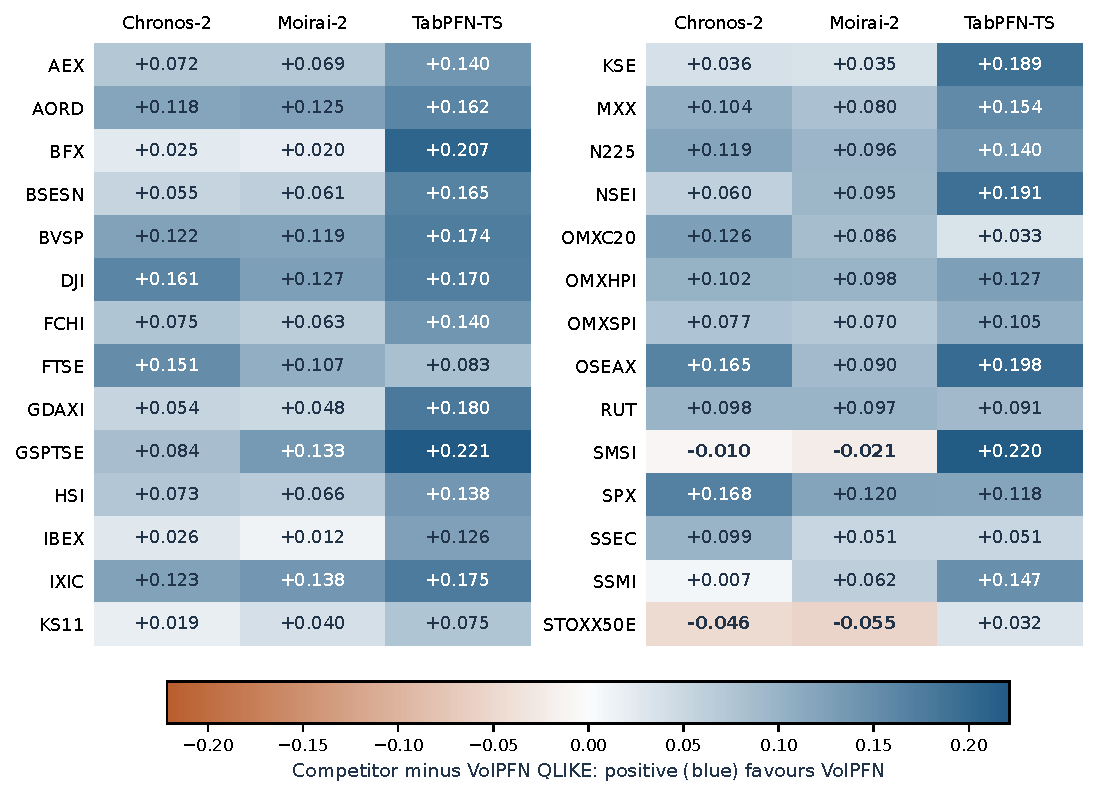
\includegraphics[width=\textwidth]{forecasting_benchmark_markets.pdf}
\caption[Corrected benchmark gains in every market]{Five-model mean competitor-minus-VolPFN QLIKE by market on the same fixed-scale benchmark panel. Blue means lower loss for VolPFN; orange means the competitor performs better. All 28 markets are shown alphabetically in two blocks. Entries are descriptive averages, not separate market-level significance tests.}
\label{fig:benchmark-market-heatmap}
\end{figure}

Historical GARCH-$t$ fits a constant mean, GARCH$(1,1)$ coefficients and tail thickness on the latest 1,000 observations, refits every 250, and updates states between fits. Seven or eight later-period refits occur per market; a failure stops the comparison rather than removing dates. UniVol uses twelve gains, five Student laws and four leverage coefficients, with restart experts favouring recent history. EWMA is initialised before scoring. These schedules are tested choices rather than established optima.

\begin{figure}[!htbp]
\centering
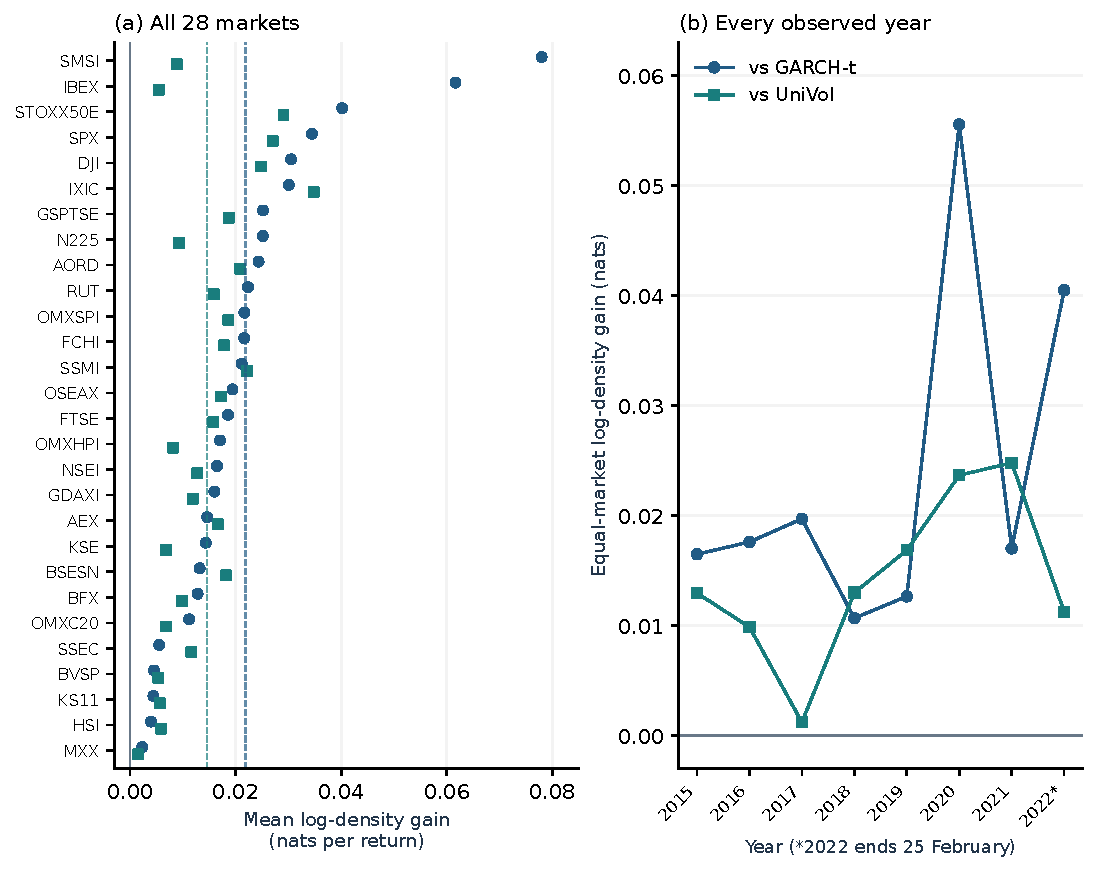
\includegraphics[width=\textwidth]{forecasting_historical_breakdown.pdf}
\caption[Where and when the historical density advantage appears]{Retained-checkpoint native log-density gains, 2015--25 February 2022. Left: all 28 market means, sorted by gain over GARCH-$t$; dashed lines are the two equal-market panel means. Right: every observed calendar year, averaging dates within each market and then markets equally. The partial 2022 period is marked. These descriptive breakdowns use existing scores and introduce no new significance tests.}
\label{fig:historical-breakdown}
\end{figure}

These selected tables complement the complete added-study comparisons in Appendix~\ref{sec:new-research-results}. Each retains its own model identity and statistical family.

\begin{table}[!htbp]\centering
\begingroup\small\setlength{\tabcolsep}{4pt}
\caption[Scores for daily financial neural predictors]{Complete daily neural procedures, 28 markets and 50,073 rows per seed, 2015--February 2022. Five seed losses receive equal weight. Squared-return QLIKE uses second moment; common-$t_8$ NLL fixes shape and native NLL uses the issued density. Lower is better.}\label{tab:new-daily-scores}
\begin{tabular}{@{}lrrr@{}}
\toprule
Procedure & $r^2$ QLIKE & Common-$t_8$ NLL & Native NLL \\
\midrule
Full VolPFN & 0.590700 & 1.184313 & 1.178272 \\
ARCH-LSTM & 0.966913 & 1.349906 & 1.268911 \\
GARCH-LSTM & 0.661074 & 1.217295 & 1.208403 \\
GINN & 0.637127 & 1.205744 & 1.204040 \\
\bottomrule
\end{tabular}\endgroup\end{table}

\begin{table}[!htbp]\centering
\begingroup\small\setlength{\tabcolsep}{4pt}
\caption[Selected common-period daily scores]{Selected raw daily-return procedures on the identical 22,026 keys, 2019--February 2022. Squared-return scoring uses second moment and RK scoring uses central variance. The full 30 September arm is the registered reference. Other daily rows, older versions and ablations remain in Appendix~\ref{sec:new-research-results}; this selection is not a claim of supported superiority over every row.}\label{tab:new-daily-common}
\begin{tabular}{@{}>{\raggedright\arraybackslash}p{6.5cm}rrr@{}}
\toprule
Procedure & $r^2$ QLIKE & RK QLIKE & Seeds \\
\midrule
Full VolPFN (30 September) & 0.703714 & 0.625668 & 5 \\
GJR-GARCH-$t$ & 0.718424 & 0.634702 & 1 \\
APARCH-$t$ & 0.722381 & 0.642651 & 1 \\
GARCH-$t$ & 0.740170 & 0.656740 & 1 \\
GINN & 0.748601 & 0.673846 & 5 \\
UniVol & 0.754697 & 0.681621 & 1 \\
GARCH-LSTM & 0.765202 & 0.710314 & 5 \\
EWMA & 0.770326 & 0.695458 & 1 \\
TabPFN-TS & 0.866181 & 0.760323 & 1 \\
ARCH-LSTM & 1.052799 & 1.021653 & 5 \\
\bottomrule
\end{tabular}\endgroup\end{table}

\begin{table}[!htbp]\centering
\begingroup\small\setlength{\tabcolsep}{4pt}
\caption[Selected realised-risk scores]{Selected realised-risk procedures, 22,026 common keys in 2019--February 2022. These have different information and fitting opportunities. Return-moment inputs use M2 for $r^2$ and variance for RK; native RK procedures use their issued risk level. Proxy-specific blends are fitted separately. GNNHAR's lower mean is included; these descriptive rows do not identify supported superiority.}\label{tab:new-intraday}
\begin{tabular}{@{}>{\raggedright\arraybackslash}p{6.5cm}rrr@{}}
\toprule
Procedure & $r^2$ QLIKE & RK QLIKE & Seeds \\
\midrule
GNNHAR adaptation & 0.669351 & 0.594805 & 5 \\
Full VolPFN+TTM-RK & 0.672139 & 0.598944 & 5 \\
GJR-GARCH-$t$+TTM-RK & 0.675318 & 0.601493 & 1 \\
QLIKE-HAR & 0.678331 & 0.599113 & 1 \\
Transfer-XGBoost & 0.693250 & 0.607646 & 5 \\
TTM-RK & 0.676869 & 0.611457 & 1 \\
Log-HAR & 0.686607 & 0.612740 & 1 \\
MS-HAR & 0.698336 & 0.623273 & 1 \\
Log-Rough-HAR & 0.710735 & 0.656406 & 1 \\
\bottomrule
\end{tabular}\endgroup\end{table}

\FloatBarrier

\section{Supplementary checks of the predictive explanation}
\label{sec:supplementary-analysis}

The supporting studies retain their development, fitting and checkpoint identities. They extend interpretation of compact recovery without providing new confirmation of the five-pair prior experiment.

\subsection{Which part of the short rule matters?}

We keep the asymmetric core fixed while adding horizons, interactions or both. Absolute-level alternatives are measured relative to initial market scale, preventing arbitrary return units from favouring relative-scale terms.

Table~\ref{tab:driver-results} uses $S_t$, the latest squared return divided by predicted risk minus one, and $d_2$, the standardised log difference between the 20- and 100-observation exponential averages. Multiplying them changes shock responsiveness; adding $d_2$ changes risk without needing a large current shock. The comparison examines these attained responses subject to fitting outcomes.

\begin{table}[!htbp]
\centering
\caption[State-variable comparisons]{Selected driver comparisons under likelihood estimation. Differences are common-$t_8$ log scores on the omitted geographical groups. All intervals are conditional development intervals; unequal optimiser convergence prevents an optimised class ordering.}
\label{tab:driver-results}
\small
\begin{tabular}{p{0.47\textwidth}rrr}
\toprule
Candidate minus comparator & Difference & 95\% interval & Markets \\
\midrule
Additive horizon terms minus asymmetric core & $+0.00310$ & $[0.00061,0.00538]$ & 23/28 \\
Shock--horizon interactions minus asymmetric core & $+0.00012$ & $[-0.00076,0.00091]$ & 13/28 \\
Full rule minus asymmetric core & $+0.00325$ & $[0.00082,0.00551]$ & 24/28 \\
$S_td_2$ minus current-scale interaction & $+0.00055$ & $[0.00019,0.00094]$ & 21/28 \\
$S_td_2$ minus long-level interaction & $+0.00040$ & $[0.00005,0.00078]$ & 22/28 \\
\bottomrule
\end{tabular}
\end{table}

The additive horizon rule retains 81.4\% of the network advantage, compared with 52.3\% for interactions and 82.8\% for the full rule. The latter is a different fit from the earlier 82.9\% result. Table~\ref{tab:driver-results} gives a positive conditional interval for direct adjustment and an interval crossing zero for interactions alone. Selected relative-scale fits outperform two absolute-level alternatives under the recorded Holm adjustment, with adjusted tail areas 0.002 and 0.023, but neither reaches the materiality criterion. These selected single-interaction fits converge without establishing global optima.

Unequal optimisation qualifies the recovery comparison. Only 57 of 68 likelihood fits and 45 of 68 path fits converge. Across four geographical likelihood folds, additive-only and asymmetric-core fits all converge, but interaction-only fails in Europe and Asia-Pacific and the full rule fails in Asia-other. Selected single relative-scale and absolute-level interaction fits converge in every fold; the separate three-level absolute interaction fails in all four. Consequently, 81.4\% versus 52.3\% describes attained-budget performance rather than optimised classes. The claim of intrinsic or optimal additive superiority remains withdrawn. The positive additive gain over the converged core still supports useful horizons, while a fair comparison of achievable driver-class performance would require a matched continued refit absent from these scores.



Figure~\ref{fig:compact-components} distinguishes attained recovery from the additive-horizon gain. Appendix~\ref{app:analysis-support} retains further fitting limits, and shock-dependent sensitivity remains possible more generally.


\subsection{Checking the role of the fitting objective}

STES provides an established alternative that uses predictors to change the weight on the latest squared return \citep{taylor2004smooth,ho2022stes}. Horizon information therefore alters responsiveness rather than adding a level adjustment. Our daily-return adaptation uses the latest square, five- and 22-observation averages, and log-level/log-ratio variants; it does not replicate an intraday-realised-variance implementation.

For each market, we fit pre-2011 observations using mean squared error (MSE) or Student likelihood, then evaluate development dates. Mean absolute error (MAE) is another reported measure. This differs from geographical coefficient transfer. Noisy squared returns and alternative losses weight large shocks differently \citep{patton2011volatility}, so failure under one objective cannot establish that an input is unhelpful under every objective.

\begin{table}[!htbp]
\centering
\caption[Smooth-transition smoothing comparisons]{STES comparisons that determine the interpretation. Except for the first row, differences are in common-$t_8$ log density. The first row uses negative absolute error, so positive differences consistently favour the candidate.}
\label{tab:stes-results}
\small
\begin{tabular}{>{\raggedright\arraybackslash}p{0.37\textwidth}>{\raggedright\arraybackslash}p{0.17\textwidth}rr}
\toprule
Candidate minus comparator & Fit; evaluation & Difference & 95\% interval \\
\midrule
Daily/weekly/monthly proxies minus daily square & MSE; $-$MAE & $-0.02411$ & $[-0.03134,-0.01742]$ \\
Daily/weekly/monthly proxies minus daily square & MSE; log score & $-0.02052$ & $[-0.02403,-0.01680]$ \\
Daily/weekly/monthly proxies minus daily square & Likelihood; log score & $+0.00039$ & $[-0.00072,0.00153]$ \\
20/100 log ratio minus daily square & Likelihood; log score & $+0.00315$ & $[0.00110,0.00534]$ \\
20/100 log ratio minus 22-day log level & Likelihood; log score & $+0.00068$ & $[-0.00124,0.00292]$ \\
\bottomrule
\end{tabular}
\end{table}

Likelihood fitting removes the large disadvantage of the daily/weekly/monthly transition set without establishing a positive reversal. The 20/100 ratio improves on the daily-square input in 27 markets, but not conclusively over the 22-day log level, leaving the joint rule unmet. Further development contrasts favour 20/100 over 5/22 by 0.00260 nats, with interval $[0.00044,0.00484]$. Freeing its two log-level coefficients gives $-0.00053$ relative to the ratio, with interval $[-0.00118,0.00010]$. All 1,008 expanded fits converge. These attained comparisons show horizon sensitivity, while successive development tests do not independently confirm a unique ratio mechanism.

\subsection{Supporting evidence from earlier prior restrictions}

The earlier smaller-network study compares broad, random-GARCH and fixed-Gaussian priors with architecture, head, auxiliary weight, lengths, overlays and 6,000 updates shared. Final checkpoints avoid selection on validation mixtures favouring broad training.

Fixing GARCH parameters at $(0.03,0.05,0.92)$ and innovations to Gaussian gives the narrowest prior. It restricts diversity and shock law together while retaining observation modifications, making this another combined-design comparison. The positive control requires broad training to improve on UniVol by 0.005 nats before narrower alternatives are interpreted.

\begin{table}[!htbp]
\centering
\caption[Completed prior-ablation runs]{Completed smaller-network ablations: common-$t_8$ advantage over UniVol, in nats per return. Seed 4 is an additional broad-prior run, not a replacement paired observation for seed 3.}
\label{tab:prior-ablation}
\small
\begin{tabular}{lrrrr}
\toprule
Training prior & Seed 1 & Seed 2 & Seed 3 & Seed 4 \\
\midrule
Broad & $+0.00555$ & $+0.00738$ & Failed & $+0.00604$ \\
Random-parameter GARCH & $-0.00292$ & $-0.00155$ & $-0.00235$ & --- \\
Fixed Gaussian GARCH & $-0.01056$ & $-0.00988$ & $-0.00837$ & --- \\
\bottomrule
\end{tabular}
\end{table}

Completed broad runs pass the control, whereas GARCH-only runs have negative panel advantages. Broad seed 3 fails on a nonfinite simulated return, and seed 4 adds an unpaired run rather than replacing it. Only two genuine broad-versus-narrow pairs remain, with mean gains 0.00870 over random GARCH and 0.01669 over fixed Gaussian. Random-minus-fixed uses three pairs and averages 0.00733. All completed paired differences are positive with individual date intervals excluding zero; those intervals do not include training-seed uncertainty.

These completed pairs favour broader simulation under the smaller budget, while the incomplete battery leaves the base-scale comparison unresolved. A separate output regression finds horizon terms even after fixed-Gaussian training. Preprocessing, architecture, overlays and correlated predictors may produce these terms, preventing their unique attribution to the broad prior. That negative attribution finding remains relevant to the later matched result.



\subsection{Details for interpreting the primary findings}
\label{sec:prior-interpretation-details}

% CLARITY PRECISION TABLE BEGIN
\begin{table}[H]
\centering\small
\caption[Recorded precision for values rounded in prose]{Previously reported values retained at their recorded precision. The scale--shape substitution averages both replacement orders for the earlier checkpoint's development comparison with UniVol. The concentration measure uses the matched prior test, and the recovery denominator uses the original compact study. These values belong to distinct studies; no new calculation is introduced.}
\label{tab:clarity-precision}
\begin{tabular}{lr}
\toprule
Quantity & Recorded value \\
\midrule
Substitution contribution from scale (nats) & 0.00778 \\
Substitution contribution from standardised shape (nats) & 0.00433 \\
Three largest markets' share of net prior gain & 50.6\% \\
Compact recovery denominator (nats) & 0.01025356 \\
\bottomrule
\end{tabular}
\end{table}
% CLARITY PRECISION TABLE END

Single-market omissions give matched-prior gains from 0.00414 to 0.00555 nats; removing the three largest contributors jointly leaves about 0.00301. These are post-result descriptive summaries, without new uncertainty intervals.

The matched prior equivalence interval is $[0.0024642,0.0076740]$, outside the declared $\pm0.003$ band. Its superiority analysis uses 5,000 resamples and 60-date blocks conditional on the ten fitted models. In the separate component programme, historical mean QLIKE is 221.292094 against 0.590118 for synthetic noaux; the gain is 220.701975 with interval $[168.500456,263.777505]$ and adjusted $p=0.000150$. The historical median is about 0.554, and 15,163 of 250,365 seed-level forecasts have QLIKE above 100. The original secondary RK diagnostic uses M2 and differs from the harmonised central-variance score. These original historical losses remain preserved diagnostics; the completed development-selected comparator in Section~\ref{sec:improved-historical} supersedes them as the principal training-source evidence.

The nine-parameter distillation rule's one-step gain over UniVol is 0.00765 nats with interval $[0.00543,0.00979]$; path gain is 0.00652 with interval $[0.00445,0.00861]$. These concern the original compression study, not the expanded driver fits. Convergence does not establish global optimality.

In synthetic tracking, the worst within-window ratio to the numerical reference is 2.14 for sparse settings against a 1.5 threshold, and 1.91 for dense settings against 1.3. The worst sparse ratio to restart experts is 1.17. The proposed sufficiently steep beyond-window deterioration also fails its recorded rule. The earlier rate classification based on goodness-of-fit values for differently transformed responses is withdrawn: such values do not distinguish logarithmic from polynomial growth. The reference uses the known law and initial state with support based on the largest visited state; support checks establish no uniform error bound. The hindsight fixed filter has additional outcome information, and only seven of eighteen simulation-fitted explicit rules converge.
\FloatBarrier

\section{Evidence locations and reproduction}
\label{sec:evidence-locations}

Portable summaries and figure inputs are held in \path{audit/} and \path{research_evidence/}. Full density, compact-rule, tracking and tail records remain in the research archives. The source README and archived unabridged appendices document paths, commands and chronology. Reconstruction from saved losses cannot recover every intermediate forecast or establish that numerical constraints never activate.

\section{Complete results for the added research}
\label{sec:new-research-results}

Each table retains its study's eligibility mask, reference and comparison family. Ordinary intervals, family intervals and seed ranges answer different questions and remain separately labelled.

\subsection{Full-period programme and the failed historical arm}

\begin{table}[H]\centering
\begingroup\small\setlength{\tabcolsep}{4pt}
\caption[All training-configuration scores]{All seven programme arms on the full 2015--February 2022 population. The secondary RK score uses second moment and its own 50,054-row-per-seed mask; it must not be substituted for the later central-variance RK score. Direct has no native density. Lower losses are preferred.}\label{tab:new-all-programme}
\begin{tabular}{@{}>{\raggedright\arraybackslash}p{3.3cm}rrrr@{}}
\toprule
Procedure & $r^2$ QLIKE & Common $t_8$ & Native NLL & RK (M2) \\
\midrule
Full VolPFN & 0.590700 & 1.184313 & 1.178272 & 0.511232 \\
Noaux & 0.590118 & 1.183908 & 1.177252 & 0.510703 \\
Direct second moment & 0.599658 & 1.188399 & --- & 0.512668 \\
Historical training & 221.292094 & 2.893771 & 33.109706 & 194.478753 \\
ARCH-LSTM & 0.966913 & 1.349906 & 1.268911 & 0.930030 \\
GARCH-LSTM & 0.661074 & 1.217295 & 1.208403 & 0.600828 \\
GINN & 0.637127 & 1.205744 & 1.204040 & 0.556977 \\
\bottomrule
\end{tabular}\endgroup\end{table}

\begin{table}[H]\centering
\begingroup\footnotesize\setlength{\tabcolsep}{3pt}
\caption[Training-component gains by seed]{Individual programme seeds: equal-market squared-return QLIKE on the complete 2015--February 2022 population. Rows are separate models, not ensembles.}\label{tab:new-programme-seeds}
\begin{tabular}{@{}lrrrrrrr@{}}
\toprule
Seed & Full & Noaux & Direct & Historical & ARCH-LSTM & GARCH-LSTM & GINN \\
\midrule
8101 & 0.591322 & 0.590379 & 0.601184 & 175.556160 & 0.965816 & 0.649599 & 0.637093 \\
8102 & 0.590656 & 0.587933 & 0.597818 & 201.027320 & 0.969667 & 0.671457 & 0.635955 \\
8103 & 0.589893 & 0.590018 & 0.604661 & 241.386418 & 0.964629 & 0.651213 & 0.642117 \\
8104 & 0.591311 & 0.590699 & 0.598014 & 297.314084 & 0.965232 & 0.659670 & 0.632799 \\
8105 & 0.590316 & 0.591563 & 0.596613 & 191.176486 & 0.969221 & 0.673432 & 0.637670 \\
\bottomrule
\end{tabular}\endgroup\end{table}

\begingroup\footnotesize\setlength{\tabcolsep}{3pt}
\begin{longtable}{@{}lrrrrrrr@{}}
\caption[Training-component gains by market]{Market means for the component and dedicated daily study, 2015--February 2022. Values average five seed losses within each market. Unequal record lengths do not weight the panel mean. The large historical losses are retained.}\label{tab:new-programme-markets}\\
\toprule
Market & Full & Noaux & Direct & Historical & ARCH & GARCH & GINN \\
\midrule\endfirsthead
\toprule
Market & Full & Noaux & Direct & Historical & ARCH & GARCH & GINN \\
\midrule\endhead
AEX & 0.307995 & 0.306063 & 0.322902 & 224.895262 & 0.736341 & 0.369218 & 0.361762 \\
AORD & 0.505451 & 0.504763 & 0.515767 & 194.176219 & 0.671421 & 0.526023 & 0.535050 \\
BFX & 0.415439 & 0.415061 & 0.418987 & 555.574760 & 0.681943 & 0.440432 & 0.459312 \\
BSESN & 0.595804 & 0.596475 & 0.609197 & 76.669727 & 1.034018 & 0.692721 & 0.629544 \\
BVSP & 0.981502 & 0.983121 & 0.985838 & 226.666016 & 1.333499 & 1.061347 & 1.040994 \\
DJI & 0.261692 & 0.260164 & 0.274401 & 177.602068 & 0.807717 & 0.378182 & 0.358568 \\
FCHI & 0.500187 & 0.497901 & 0.514031 & 581.534543 & 0.863135 & 0.554966 & 0.556809 \\
FTSE & 0.731466 & 0.731983 & 0.746558 & 139.500838 & 1.020572 & 0.774449 & 0.781394 \\
GDAXI & 0.695488 & 0.693904 & 0.715287 & 126.800414 & 1.035813 & 0.751182 & 0.748027 \\
GSPTSE & -0.216739 & -0.217893 & -0.206891 & 192.013638 & 0.378635 & -0.035425 & -0.117972 \\
HSI & 0.650265 & 0.651581 & 0.650462 & 160.671346 & 0.812766 & 0.668526 & 0.672647 \\
IBEX & 0.687386 & 0.685351 & 0.687539 & 299.716951 & 1.028851 & 0.713983 & 0.712204 \\
IXIC & 0.653567 & 0.653139 & 0.669081 & 336.419421 & 1.170668 & 0.739529 & 0.717200 \\
KS11 & 0.200748 & 0.202232 & 0.201809 & 202.451337 & 0.805178 & 0.350308 & 0.245721 \\
KSE & 0.810501 & 0.807684 & 0.818471 & 136.702667 & 1.119874 & 0.870487 & 0.851475 \\
MXX & 0.628318 & 0.628994 & 0.628110 & 175.026482 & 1.023769 & 0.680181 & 0.633288 \\
N225 & 0.530539 & 0.531215 & 0.536371 & 199.611627 & 0.884572 & 0.623965 & 0.598585 \\
NSEI & 0.558244 & 0.557847 & 0.578476 & 245.116532 & 0.876870 & 0.587450 & 0.585291 \\
OMXC20 & 0.991254 & 0.989308 & 1.003431 & 189.654288 & 1.181254 & 1.017881 & 1.013313 \\
OMXHPI & 0.491254 & 0.491342 & 0.502571 & 165.768945 & 1.053381 & 0.641089 & 0.557585 \\
OMXSPI & 0.438294 & 0.436547 & 0.447499 & 180.050416 & 1.085286 & 0.586040 & 0.482323 \\
OSEAX & 0.920134 & 0.918636 & 0.941834 & 160.015300 & 1.179178 & 0.994276 & 0.972340 \\
RUT & 0.993527 & 0.994288 & 1.002787 & 170.932093 & 1.169371 & 1.024047 & 1.012883 \\
SMSI & 0.822091 & 0.820251 & 0.816680 & 205.204763 & 1.076206 & 0.843808 & 0.846751 \\
SPX & 0.223903 & 0.223274 & 0.238277 & 222.671830 & 0.804136 & 0.342858 & 0.340832 \\
SSEC & 0.994067 & 0.994996 & 0.989708 & 191.561889 & 1.413150 & 1.060551 & 1.004844 \\
SSMI & 0.365734 & 0.365701 & 0.359111 & 161.854790 & 0.620202 & 0.384701 & 0.369079 \\
STOXX50E & 0.801475 & 0.799389 & 0.822131 & 297.314457 & 1.205750 & 0.867301 & 0.869703 \\
\bottomrule
\end{longtable}\endgroup


We average scores across dates within each market, then give markets and seeds equal weight. Each seed is scored separately; the forecasts are not ensembled. The original fixed-final historical arm remains as a diagnostic; Section~\ref{sec:improved-historical} supplies the stronger completed comparator and Appendix~\ref{sec:followup-results} its separate inference. Maximum QLIKE is about 3.72 million and minimum issued second moment about $1.09\times10^{-6}$. All four configurations share one-position extrapolation: the largest trained prediction position is 1022, while evaluation reaches 1023. Neither pinned replay nor these diagnostics establish a sole failure cause.

\subsection{Common-period daily evidence}

\begingroup\small\setlength{\tabcolsep}{4pt}
\begin{longtable}{@{}>{\raggedright\arraybackslash}p{6.5cm}rrr@{}}
\caption[Complete common-period daily scores]{Complete saved daily table and supplementary configurations, 22,026 keys in 2019--February 2022. The 26 September model and ablations retain distinct identities. RK scoring uses central variance; direct RK is unavailable. Descriptive loss ordering does not transfer tests between model versions.}\label{tab:new-daily-common-all}\\
\toprule
Procedure & $r^2$ QLIKE & RK QLIKE & Seeds \\
\midrule\endfirsthead
\toprule
Procedure & $r^2$ QLIKE & RK QLIKE & Seeds \\
\midrule\endhead
VolPFN (26 September) & 0.703689 & 0.625397 & 5 \\
Full VolPFN (30 September) & 0.703714 & 0.625668 & 5 \\
GJR-GARCH-$t$ & 0.718424 & 0.634702 & 1 \\
APARCH-$t$ & 0.722381 & 0.642651 & 1 \\
GARCH-$t$ & 0.740170 & 0.656740 & 1 \\
GINN & 0.748601 & 0.673846 & 5 \\
UniVol & 0.754697 & 0.681621 & 1 \\
GARCH-LSTM & 0.765202 & 0.710314 & 5 \\
EWMA & 0.770326 & 0.695458 & 1 \\
TabPFN-TS & 0.866181 & 0.760323 & 1 \\
ARCH-LSTM & 1.052799 & 1.021653 & 5 \\
Historical variance (250) & 1.072036 & 1.076967 & 1 \\
EGARCH-$t$ & 2.376730 & 2.303764 & 1 \\
Chronos-2 & 2.478397 & 2.191879 & 1 \\
Moirai-2 & $7.03773\times10^{5}$ & $1.30930\times10^{6}$ & 1 \\
TTM square-root RK diagnostic & 0.687005 & 0.607298 & 1 \\
Noaux & 0.702624 & 0.624696 & 5 \\
Compact nine-parameter rule & 0.705530 & 0.642068 & 1 \\
Direct second moment & 0.712596 & --- & 5 \\
Mean-log HAR diagnostic & 0.713198 & 0.663236 & 1 \\
Historical training & 222.674179 & $1.92096\times10^{4}$ & 5 \\
\bottomrule
\end{longtable}\endgroup

\begingroup\footnotesize\setlength{\tabcolsep}{2pt}
\begin{longtable}{@{}>{\raggedright\arraybackslash}p{2.0cm}lrccr@{}}
\caption[Complete common-period daily inference]{All primary-block contrasts in the separate 28-slot daily family, full 30 September reference. Gains are comparator minus reference. Ordinary and Bonferroni family intervals are distinct; joint support also requires both proxies and all reference-seed directions.}\label{tab:new-daily-inference}\\
\toprule
Comparator & Proxy & Gain & Ordinary 95\% & Family 95\% & Holm $p$ \\
\midrule\endfirsthead
\toprule
Comparator & Proxy & Gain & Ordinary 95\% & Family 95\% & Holm $p$ \\
\midrule\endhead
VolPFN (26 September) & $r^2$ & -0.000025 & $[-0.000511,0.000456]$ & $[-0.000806,0.000699]$ & 0.922604 \\
VolPFN (26 September) & RK & -0.000271 & $[-0.000614,0.000056]$ & $[-0.000841,0.000228]$ & 0.644468 \\
GJR-GARCH-$t$ & $r^2$ & 0.014710 & $[0.002690,0.025596]$ & $[-0.005585,0.030755]$ & 0.185241 \\
GJR-GARCH-$t$ & RK & 0.009034 & $[0.000203,0.016813]$ & $[-0.005703,0.020749]$ & 0.395980 \\
APARCH-$t$ & $r^2$ & 0.018667 & $[-0.007799,0.036714]$ & $[-0.028895,0.041415]$ & 0.644468 \\
APARCH-$t$ & RK & 0.016983 & $[-0.009022,0.033151]$ & $[-0.030504,0.037170]$ & 0.644468 \\
GARCH-$t$ & $r^2$ & 0.036456 & $[0.002342,0.060043]$ & $[-0.025383,0.066577]$ & 0.245038 \\
GARCH-$t$ & RK & 0.031072 & $[-0.003685,0.052449]$ & $[-0.031830,0.056857]$ & 0.447678 \\
GINN & $r^2$ & 0.044887 & $[0.021849,0.066686]$ & $[0.007220,0.079608]$ & 0.002000 \\
GINN & RK & 0.048178 & $[0.020320,0.067348]$ & $[-0.001748,0.073965]$ & 0.020399 \\
UniVol & $r^2$ & 0.050984 & $[0.031216,0.067877]$ & $[0.018917,0.076424]$ & 0.001400 \\
UniVol & RK & 0.055953 & $[0.033186,0.073476]$ & $[0.017825,0.080113]$ & 0.002000 \\
GARCH-LSTM & $r^2$ & 0.061488 & $[0.038481,0.085014]$ & $[0.023466,0.099624]$ & 0.001400 \\
GARCH-LSTM & RK & 0.084646 & $[0.062228,0.105809]$ & $[0.048995,0.117452]$ & 0.001400 \\
EWMA & $r^2$ & 0.066612 & $[0.011440,0.106244]$ & $[-0.031369,0.121346]$ & 0.184791 \\
EWMA & RK & 0.069790 & $[0.008943,0.110205]$ & $[-0.035559,0.119373]$ & 0.200190 \\
TabPFN-TS & $r^2$ & 0.162467 & $[0.127795,0.191350]$ & $[0.103711,0.203598]$ & 0.001400 \\
TabPFN-TS & RK & 0.134655 & $[0.112725,0.154649]$ & $[0.098722,0.164135]$ & 0.001400 \\
ARCH-LSTM & $r^2$ & 0.349085 & $[0.252951,0.448091]$ & $[0.195952,0.508750]$ & 0.001400 \\
ARCH-LSTM & RK & 0.395985 & $[0.295073,0.492363]$ & $[0.240872,0.547212]$ & 0.001400 \\
Historical variance (250) & $r^2$ & 0.368323 & $[-0.115800,0.635827]$ & $[-0.541047,0.668407]$ & 0.644468 \\
Historical variance (250) & RK & 0.451299 & $[-0.167356,0.780805]$ & $[-0.698921,0.809609]$ & 0.644468 \\
EGARCH-$t$ & $r^2$ & 1.673016 & $[-0.833468,3.312847]$ & $[-2.614018,3.345017]$ & 0.644468 \\
EGARCH-$t$ & RK & 1.678096 & $[-0.828472,3.319278]$ & $[-2.613402,3.351321]$ & 0.644468 \\
Chronos-2 & $r^2$ & 1.774683 & $[1.019284,2.293604]$ & $[0.413181,2.430903]$ & 0.001400 \\
Chronos-2 & RK & 1.566211 & $[0.819291,2.035569]$ & $[0.184280,2.137435]$ & 0.002700 \\
Moirai-2 & $r^2$ & $7.03772\times10^{5}$ & $[-7.18415\times10^{5},1.40754\times10^{6}]$ & $[-1.94660\times10^{6},1.40754\times10^{6}]$ & 0.644468 \\
Moirai-2 & RK & $1.30930\times10^{6}$ & $[-1.33241\times10^{6},2.61859\times10^{6}]$ & $[-3.78065\times10^{6},2.61859\times10^{6}]$ & 0.644468 \\
\bottomrule
\end{longtable}\endgroup


Direct predicts second moment without a separately identified central variance. Its earlier M2/RK diagnostic therefore cannot fill the harmonised variance/RK slot. Alignment uses saved forecasts without retraining or calibration. Extreme losses describe the issued procedures rather than all members of a model family.

\subsection{Complete realised-risk and helper comparisons}

\begingroup\small\setlength{\tabcolsep}{4pt}
\begin{longtable}{@{}>{\raggedright\arraybackslash}p{6.5cm}rrr@{}}
\caption[Complete realised-risk scores]{All eighteen completed intraday-extension procedures on the common 2019--February 2022 panel. Lower is better; complete-procedure comparisons do not isolate architecture. Unavailable M2VN and DeepRGARCH retain statistical slots without fabricated scores.}\label{tab:new-intraday-all}\\
\toprule
Procedure & $r^2$ QLIKE & RK QLIKE & Seeds \\
\midrule\endfirsthead
\toprule
Procedure & $r^2$ QLIKE & RK QLIKE & Seeds \\
\midrule\endhead
Full VolPFN+TTM-RK & 0.672139 & 0.598944 & 5 \\
VolPFN (26 Sept.)+TTM-RK & 0.672203 & 0.598948 & 5 \\
Full VolPFN+Log-HAR & 0.675699 & 0.605183 & 5 \\
Full VolPFN+MS-HAR & 0.682335 & 0.609285 & 5 \\
GJR-GARCH-$t$+TTM-RK & 0.675318 & 0.601493 & 1 \\
GJR-GARCH-$t$+Log-HAR & 0.679109 & 0.607935 & 1 \\
MS-HAR+Log-HAR & 0.684291 & 0.615649 & 1 \\
Full VolPFN (30 September) & 0.703714 & 0.625668 & 5 \\
VolPFN (26 September) & 0.703689 & 0.625397 & 5 \\
GJR-GARCH-$t$ & 0.718424 & 0.634702 & 1 \\
HAR & 28.898514 & 31.530660 & 1 \\
Log-HAR & 0.686607 & 0.612740 & 1 \\
TTM-RK & 0.676869 & 0.611457 & 1 \\
MS-HAR & 0.698336 & 0.623273 & 1 \\
Log-Rough-HAR & 0.710735 & 0.656406 & 1 \\
GNNHAR adaptation & 0.669351 & 0.594805 & 5 \\
QLIKE-HAR & 0.678331 & 0.599113 & 1 \\
Transfer-XGBoost & 0.693250 & 0.607646 & 5 \\
\bottomrule
\end{longtable}\endgroup

\begingroup\footnotesize\setlength{\tabcolsep}{3pt}
\begin{longtable}{@{}>{\raggedright\arraybackslash}p{2.7cm}lrccr@{}}
\caption[Complete realised-risk inference]{All primary-block contrasts in the 38-slot intraday family, full VolPFN+TTM reference. Unavailable entries retain $p=1$. Ordinary and Bonferroni family intervals are shown separately. Joint support requires both proxies and all reference-seed directions.}\label{tab:new-intraday-inference}\\
\toprule
Comparator & Proxy & Gain & Ordinary 95\% & Family 95\% & Holm $p$ \\
\midrule\endfirsthead
\toprule
Comparator & Proxy & Gain & Ordinary 95\% & Family 95\% & Holm $p$ \\
\midrule\endhead
VolPFN (26 Sept.)+TTM-RK & $r^2$ & 0.000064 & $[-0.000097,0.000217]$ & $[-0.000198,0.000309]$ & 1.000000 \\
VolPFN (26 Sept.)+TTM-RK & RK & 0.000004 & $[-0.000124,0.000120]$ & $[-0.000208,0.000183]$ & 1.000000 \\
Full VolPFN+Log-HAR & $r^2$ & 0.003560 & $[-0.005272,0.011764]$ & $[-0.011053,0.016594]$ & 1.000000 \\
Full VolPFN+Log-HAR & RK & 0.006240 & $[-0.009361,0.016293]$ & $[-0.023389,0.019753]$ & 1.000000 \\
Full VolPFN+MS-HAR & $r^2$ & 0.010196 & $[-0.005476,0.022851]$ & $[-0.016592,0.029472]$ & 1.000000 \\
Full VolPFN+MS-HAR & RK & 0.010341 & $[-0.009719,0.022438]$ & $[-0.028138,0.025980]$ & 1.000000 \\
GJR-GARCH-$t$+TTM-RK & $r^2$ & 0.003178 & $[0.001303,0.004841]$ & $[-0.000110,0.005768]$ & 0.033598 \\
GJR-GARCH-$t$+TTM-RK & RK & 0.002549 & $[0.000988,0.003926]$ & $[-0.000122,0.004627]$ & 0.034098 \\
GJR-GARCH-$t$+Log-HAR & $r^2$ & 0.006970 & $[-0.004819,0.016608]$ & $[-0.013898,0.021992]$ & 1.000000 \\
GJR-GARCH-$t$+Log-HAR & RK & 0.008991 & $[-0.008927,0.020107]$ & $[-0.024760,0.023645]$ & 1.000000 \\
MS-HAR+Log-HAR & $r^2$ & 0.012152 & $[-0.008476,0.026574]$ & $[-0.026187,0.031898]$ & 1.000000 \\
MS-HAR+Log-HAR & RK & 0.016705 & $[-0.011499,0.033236]$ & $[-0.037620,0.036888]$ & 1.000000 \\
Full VolPFN (30 September) & $r^2$ & 0.031574 & $[0.017986,0.043996]$ & $[0.009333,0.050936]$ & 0.001900 \\
Full VolPFN (30 September) & RK & 0.026724 & $[0.020980,0.032708]$ & $[0.017644,0.036689]$ & 0.001900 \\
VolPFN (26 September) & $r^2$ & 0.031549 & $[0.017971,0.044010]$ & $[0.009263,0.050998]$ & 0.001900 \\
VolPFN (26 September) & RK & 0.026453 & $[0.020694,0.032420]$ & $[0.017357,0.036489]$ & 0.001900 \\
GJR-GARCH-$t$ & $r^2$ & 0.046284 & $[0.023908,0.066211]$ & $[0.008443,0.075818]$ & 0.001900 \\
GJR-GARCH-$t$ & RK & 0.035758 & $[0.025420,0.045467]$ & $[0.018580,0.051432]$ & 0.001900 \\
HAR & $r^2$ & 28.226375 & $[-29.377519,56.447931]$ & $[-85.062870,56.459737]$ & 1.000000 \\
HAR & RK & 30.931716 & $[-32.218364,61.854624]$ & $[-92.823133,61.860491]$ & 1.000000 \\
Log-HAR & $r^2$ & 0.014468 & $[-0.006438,0.032055]$ & $[-0.021355,0.041210]$ & 1.000000 \\
Log-HAR & RK & 0.013796 & $[-0.008934,0.028376]$ & $[-0.028989,0.033451]$ & 1.000000 \\
TTM-RK & $r^2$ & 0.004730 & $[-0.000936,0.010178]$ & $[-0.004558,0.013468]$ & 1.000000 \\
TTM-RK & RK & 0.012513 & $[0.003683,0.021801]$ & $[-0.001702,0.027669]$ & 0.173991 \\
MS-HAR & $r^2$ & 0.026197 & $[-0.003996,0.049557]$ & $[-0.027159,0.060511]$ & 1.000000 \\
MS-HAR & RK & 0.024329 & $[-0.000089,0.039808]$ & $[-0.021841,0.044643]$ & 0.684416 \\
Log-Rough-HAR & $r^2$ & 0.038596 & $[-0.036928,0.083934]$ & $[-0.103821,0.095360]$ & 1.000000 \\
Log-Rough-HAR & RK & 0.057462 & $[-0.054158,0.116379]$ & $[-0.161461,0.121709]$ & 1.000000 \\
GNNHAR adaptation & $r^2$ & -0.002788 & $[-0.017395,0.015490]$ & $[-0.024113,0.027691]$ & 1.000000 \\
GNNHAR adaptation & RK & -0.004139 & $[-0.016860,0.015021]$ & $[-0.020967,0.029546]$ & 1.000000 \\
QLIKE-HAR & $r^2$ & 0.006192 & $[-0.009076,0.022959]$ & $[-0.016646,0.032510]$ & 1.000000 \\
QLIKE-HAR & RK & 0.000170 & $[-0.011345,0.015936]$ & $[-0.015565,0.028032]$ & 1.000000 \\
Transfer-XGBoost & $r^2$ & 0.021110 & $[0.006779,0.035218]$ & $[-0.001801,0.044420]$ & 0.104995 \\
Transfer-XGBoost & RK & 0.008702 & $[0.002141,0.015354]$ & $[-0.001859,0.019703]$ & 0.282786 \\
M2VN (unavailable) & $r^2$ & --- & --- & --- & 1.000000 \\
M2VN (unavailable) & RK & --- & --- & --- & 1.000000 \\
DeepRGARCH (unavailable) & $r^2$ & --- & --- & --- & 1.000000 \\
DeepRGARCH (unavailable) & RK & --- & --- & --- & 1.000000 \\
\bottomrule
\end{longtable}\endgroup

\begin{table}[H]\centering
\begingroup\small\setlength{\tabcolsep}{4pt}
\caption[Complete cross-market-helper scores]{Cross-market-helper follow-up and preserved controls on the same 22,026 keys. All helper-containing procedures score five seed losses separately. The reference is VolPFN+helper, and no comparator passes the separate twelve-slot two-proxy rule.}\label{tab:new-helper-all}
\begin{tabular}{@{}>{\raggedright\arraybackslash}p{6.5cm}rrr@{}}
\toprule
Procedure & $r^2$ QLIKE & RK QLIKE & Seeds \\
\midrule
GNNHAR adaptation & 0.669351 & 0.594805 & 5 \\
Full VolPFN+TTM-RK & 0.672139 & 0.598944 & 5 \\
VolPFN+helper & 0.674026 & 0.603577 & 5 \\
GJR+helper & 0.677955 & 0.606815 & 5 \\
Transfer-XGBoost & 0.693250 & 0.607646 & 5 \\
Cross-market helper & 0.686927 & 0.618399 & 5 \\
Calibrated helper & 0.694879 & 0.644218 & 5 \\
\bottomrule
\end{tabular}\endgroup\end{table}

\begingroup\footnotesize\setlength{\tabcolsep}{3pt}
\begin{longtable}{@{}>{\raggedright\arraybackslash}p{2.7cm}lrccr@{}}
\caption[Cross-market-helper inference]{All primary-block contrasts in the separate twelve-slot helper family, VolPFN+helper reference. Ordinary and family intervals are distinct. Joint support requires both proxies and corresponding seed directions; no contrast meets the complete rule.}\label{tab:new-helper-inference}\\
\toprule
Comparator & Proxy & Gain & Ordinary 95\% & Family 95\% & Holm $p$ \\
\midrule\endfirsthead
\toprule
Comparator & Proxy & Gain & Ordinary 95\% & Family 95\% & Holm $p$ \\
\midrule\endhead
Calibrated helper & $r^2$ & 0.020853 & $[-0.000781,0.034324]$ & $[-0.014486,0.037312]$ & 0.207540 \\
Calibrated helper & RK & 0.040641 & $[-0.011515,0.068908]$ & $[-0.051015,0.071198]$ & 0.419679 \\
GJR+helper & $r^2$ & 0.003929 & $[0.000753,0.006443]$ & $[-0.001145,0.007410]$ & 0.093595 \\
GJR+helper & RK & 0.003238 & $[0.001269,0.004910]$ & $[0.000142,0.005580]$ & 0.019799 \\
Cross-market helper & $r^2$ & 0.012900 & $[0.004429,0.020533]$ & $[0.000455,0.023670]$ & 0.020349 \\
Cross-market helper & RK & 0.014822 & $[0.005537,0.021121]$ & $[-0.000029,0.023125]$ & 0.021499 \\
Full VolPFN+TTM-RK & $r^2$ & -0.001887 & $[-0.010294,0.006141]$ & $[-0.013763,0.009722]$ & 1.000000 \\
Full VolPFN+TTM-RK & RK & -0.004634 & $[-0.010436,0.002143]$ & $[-0.012897,0.005651]$ & 0.712464 \\
GNNHAR adaptation & $r^2$ & -0.004675 & $[-0.016137,0.008789]$ & $[-0.020064,0.016260]$ & 1.000000 \\
GNNHAR adaptation & RK & -0.008772 & $[-0.022388,0.014764]$ & $[-0.025260,0.029053]$ & 1.000000 \\
Transfer-XGBoost & $r^2$ & 0.019223 & $[0.002313,0.033344]$ & $[-0.006677,0.038430]$ & 0.130793 \\
Transfer-XGBoost & RK & 0.004068 & $[-0.003265,0.012671]$ & $[-0.006041,0.017110]$ & 1.000000 \\
\bottomrule
\end{longtable}\endgroup

\clearpage
\begin{table}[!htbp]\centering
\begingroup\small\setlength{\tabcolsep}{4pt}
\caption[Common-period reference seeds]{Equal-market descriptive seed losses on the same 22,026 keys. These are separately scored forecasts, not ensembles or independent significance tests.}\label{tab:new-common-seeds}
\begin{tabular}{@{}l>{\raggedright\arraybackslash}p{6cm}rr@{}}
\toprule
Seed & Procedure & $r^2$ QLIKE & RK QLIKE \\
\midrule
8101 & Full VolPFN+TTM-RK & 0.672112 & 0.598389 \\
8101 & GNNHAR adaptation & 0.669137 & 0.595102 \\
8101 & VolPFN+helper & 0.675812 & 0.603673 \\
8102 & Full VolPFN+TTM-RK & 0.672698 & 0.600277 \\
8102 & GNNHAR adaptation & 0.670172 & 0.594903 \\
8102 & VolPFN+helper & 0.673559 & 0.604507 \\
8103 & Full VolPFN+TTM-RK & 0.671690 & 0.598390 \\
8103 & GNNHAR adaptation & 0.670782 & 0.595442 \\
8103 & VolPFN+helper & 0.672844 & 0.602767 \\
8104 & Full VolPFN+TTM-RK & 0.672015 & 0.598924 \\
8104 & GNNHAR adaptation & 0.667610 & 0.594185 \\
8104 & VolPFN+helper & 0.674199 & 0.603934 \\
8105 & Full VolPFN+TTM-RK & 0.672181 & 0.598739 \\
8105 & GNNHAR adaptation & 0.669054 & 0.594394 \\
8105 & VolPFN+helper & 0.673718 & 0.603006 \\
\bottomrule
\end{tabular}\endgroup\end{table}

\clearpage
\begingroup\footnotesize\setlength{\tabcolsep}{3pt}
\begin{longtable}{@{}lrrrrrr@{}}
\caption[Realised-risk gains by market]{Descriptive market gains relative to VolPFN+TTM on common keys. Five seed losses are averaged where available; GJR+TTM is a single deterministic procedure. Positive favours the reference. GNN denotes GNNHAR, GJR denotes GJR+TTM and Transfer denotes Transfer-XGBoost. These market means are not separate adjusted tests.}\label{tab:new-intraday-markets}\\
\toprule
Market & GNN $r^2$ & GNN RK & GJR $r^2$ & GJR RK & Transfer $r^2$ & Transfer RK \\
\midrule\endfirsthead
\toprule
Market & GNN $r^2$ & GNN RK & GJR $r^2$ & GJR RK & Transfer $r^2$ & Transfer RK \\
\midrule\endhead
AEX & -0.004880 & 0.003499 & 0.004816 & 0.001219 & 0.005588 & 0.010200 \\
AORD & 0.011702 & -0.000012 & 0.004369 & 0.004830 & 0.026337 & 0.016252 \\
BFX & -0.028661 & -0.019229 & 0.000518 & -0.000531 & -0.020708 & -0.001484 \\
BSESN & 0.009606 & -0.006744 & 0.003066 & 0.004445 & 0.035817 & 0.006712 \\
BVSP & -0.008100 & -0.017983 & -0.002132 & -0.002900 & 0.000882 & -0.004826 \\
DJI & -0.016879 & -0.004871 & 0.001964 & 0.002608 & 0.024665 & 0.015848 \\
FCHI & -0.022963 & -0.006115 & 0.003307 & 0.000874 & -0.016859 & 0.006464 \\
FTSE & -0.026164 & -0.000944 & 0.004177 & -0.000496 & 0.011362 & 0.006281 \\
GDAXI & 0.020021 & -0.006141 & 0.005131 & 0.002833 & 0.041264 & 0.002598 \\
GSPTSE & -0.020960 & -0.000810 & 0.011588 & 0.005500 & 0.032637 & 0.024393 \\
HSI & 0.003172 & -0.010581 & 0.001861 & 0.004211 & 0.017058 & 0.000031 \\
IBEX & -0.002851 & -0.001081 & 0.005330 & 0.008744 & -0.006339 & 0.008881 \\
IXIC & -0.016576 & -0.003281 & -0.002364 & -0.000847 & 0.009439 & 0.015606 \\
KS11 & -0.019007 & 0.001445 & 0.006160 & 0.005431 & 0.010241 & 0.016196 \\
KSE & 0.014723 & -0.016338 & 0.002176 & 0.003037 & 0.041852 & -0.001262 \\
MXX & 0.019970 & -0.003170 & -0.000021 & 0.000261 & 0.030215 & 0.005832 \\
N225 & 0.003498 & -0.006222 & 0.000305 & -0.000808 & 0.029530 & 0.002777 \\
NSEI & 0.021473 & -0.003104 & 0.001778 & 0.000890 & 0.071996 & 0.019171 \\
OMXC20 & 0.011535 & -0.009548 & 0.001636 & 0.001347 & 0.025091 & -0.002972 \\
OMXHPI & 0.007281 & -0.000893 & 0.007049 & 0.003464 & 0.021098 & 0.014014 \\
OMXSPI & 0.004083 & 0.005850 & 0.003951 & 0.002451 & 0.018173 & 0.016870 \\
OSEAX & 0.009113 & -0.011555 & 0.008399 & 0.007868 & 0.036921 & -0.001453 \\
RUT & 0.004147 & 0.008881 & 0.003160 & 0.005286 & 0.033490 & 0.021941 \\
SMSI & -0.009324 & 0.008057 & -0.001772 & 0.001369 & 0.004097 & 0.009261 \\
SPX & -0.021135 & -0.001771 & 0.001413 & 0.002497 & 0.019871 & 0.017648 \\
SSEC & 0.018688 & -0.006713 & 0.001787 & 0.001090 & 0.048157 & -0.003318 \\
SSMI & -0.035504 & -0.016728 & 0.004288 & 0.004047 & -0.004587 & -0.004951 \\
STOXX50E & -0.004078 & 0.010216 & 0.007051 & 0.002662 & 0.043803 & 0.026951 \\
\bottomrule
\end{longtable}\endgroup


Both proxies must satisfy the complete registered joint rule for support. Market signs and seed ranges remain descriptive. The bundle retains block-20/120 sensitivities and complete seed and market records; inference conditions on saved forecasts without training or refitting uncertainty.

\subsection{Unavailable procedures, failures and remaining experiments}

Unavailable procedures remain visible: M2VN lacks compatible news and predictors, exact DeepRGARCH and DCC/GN-GARCH were not run, RECH is unavailable, and GP-Vol coverage is incomplete. Missing family slots retain $p=1$ without invented forecasts. We distinguish original failures from later continuations and discuss the outstanding controls and generalisation questions in Chapter~\ref{ch:discussion}.

\FloatBarrier


\section{Completed follow-ups: controls and external validation}
\label{sec:followup-results}

Chapters~\ref{ch:forecast} and \ref{ch:analysis} place these findings in the performance and training-source arguments. Here we retain exact primary summaries, seed results and sensitivity decisions. Gains are absolute QLIKE differences rather than percentage improvements. Figure~\ref{fig:followup-primary} presents their directions and uncertainty without pooling populations or multiplicity families.

\begin{figure}[!htbp]\centering
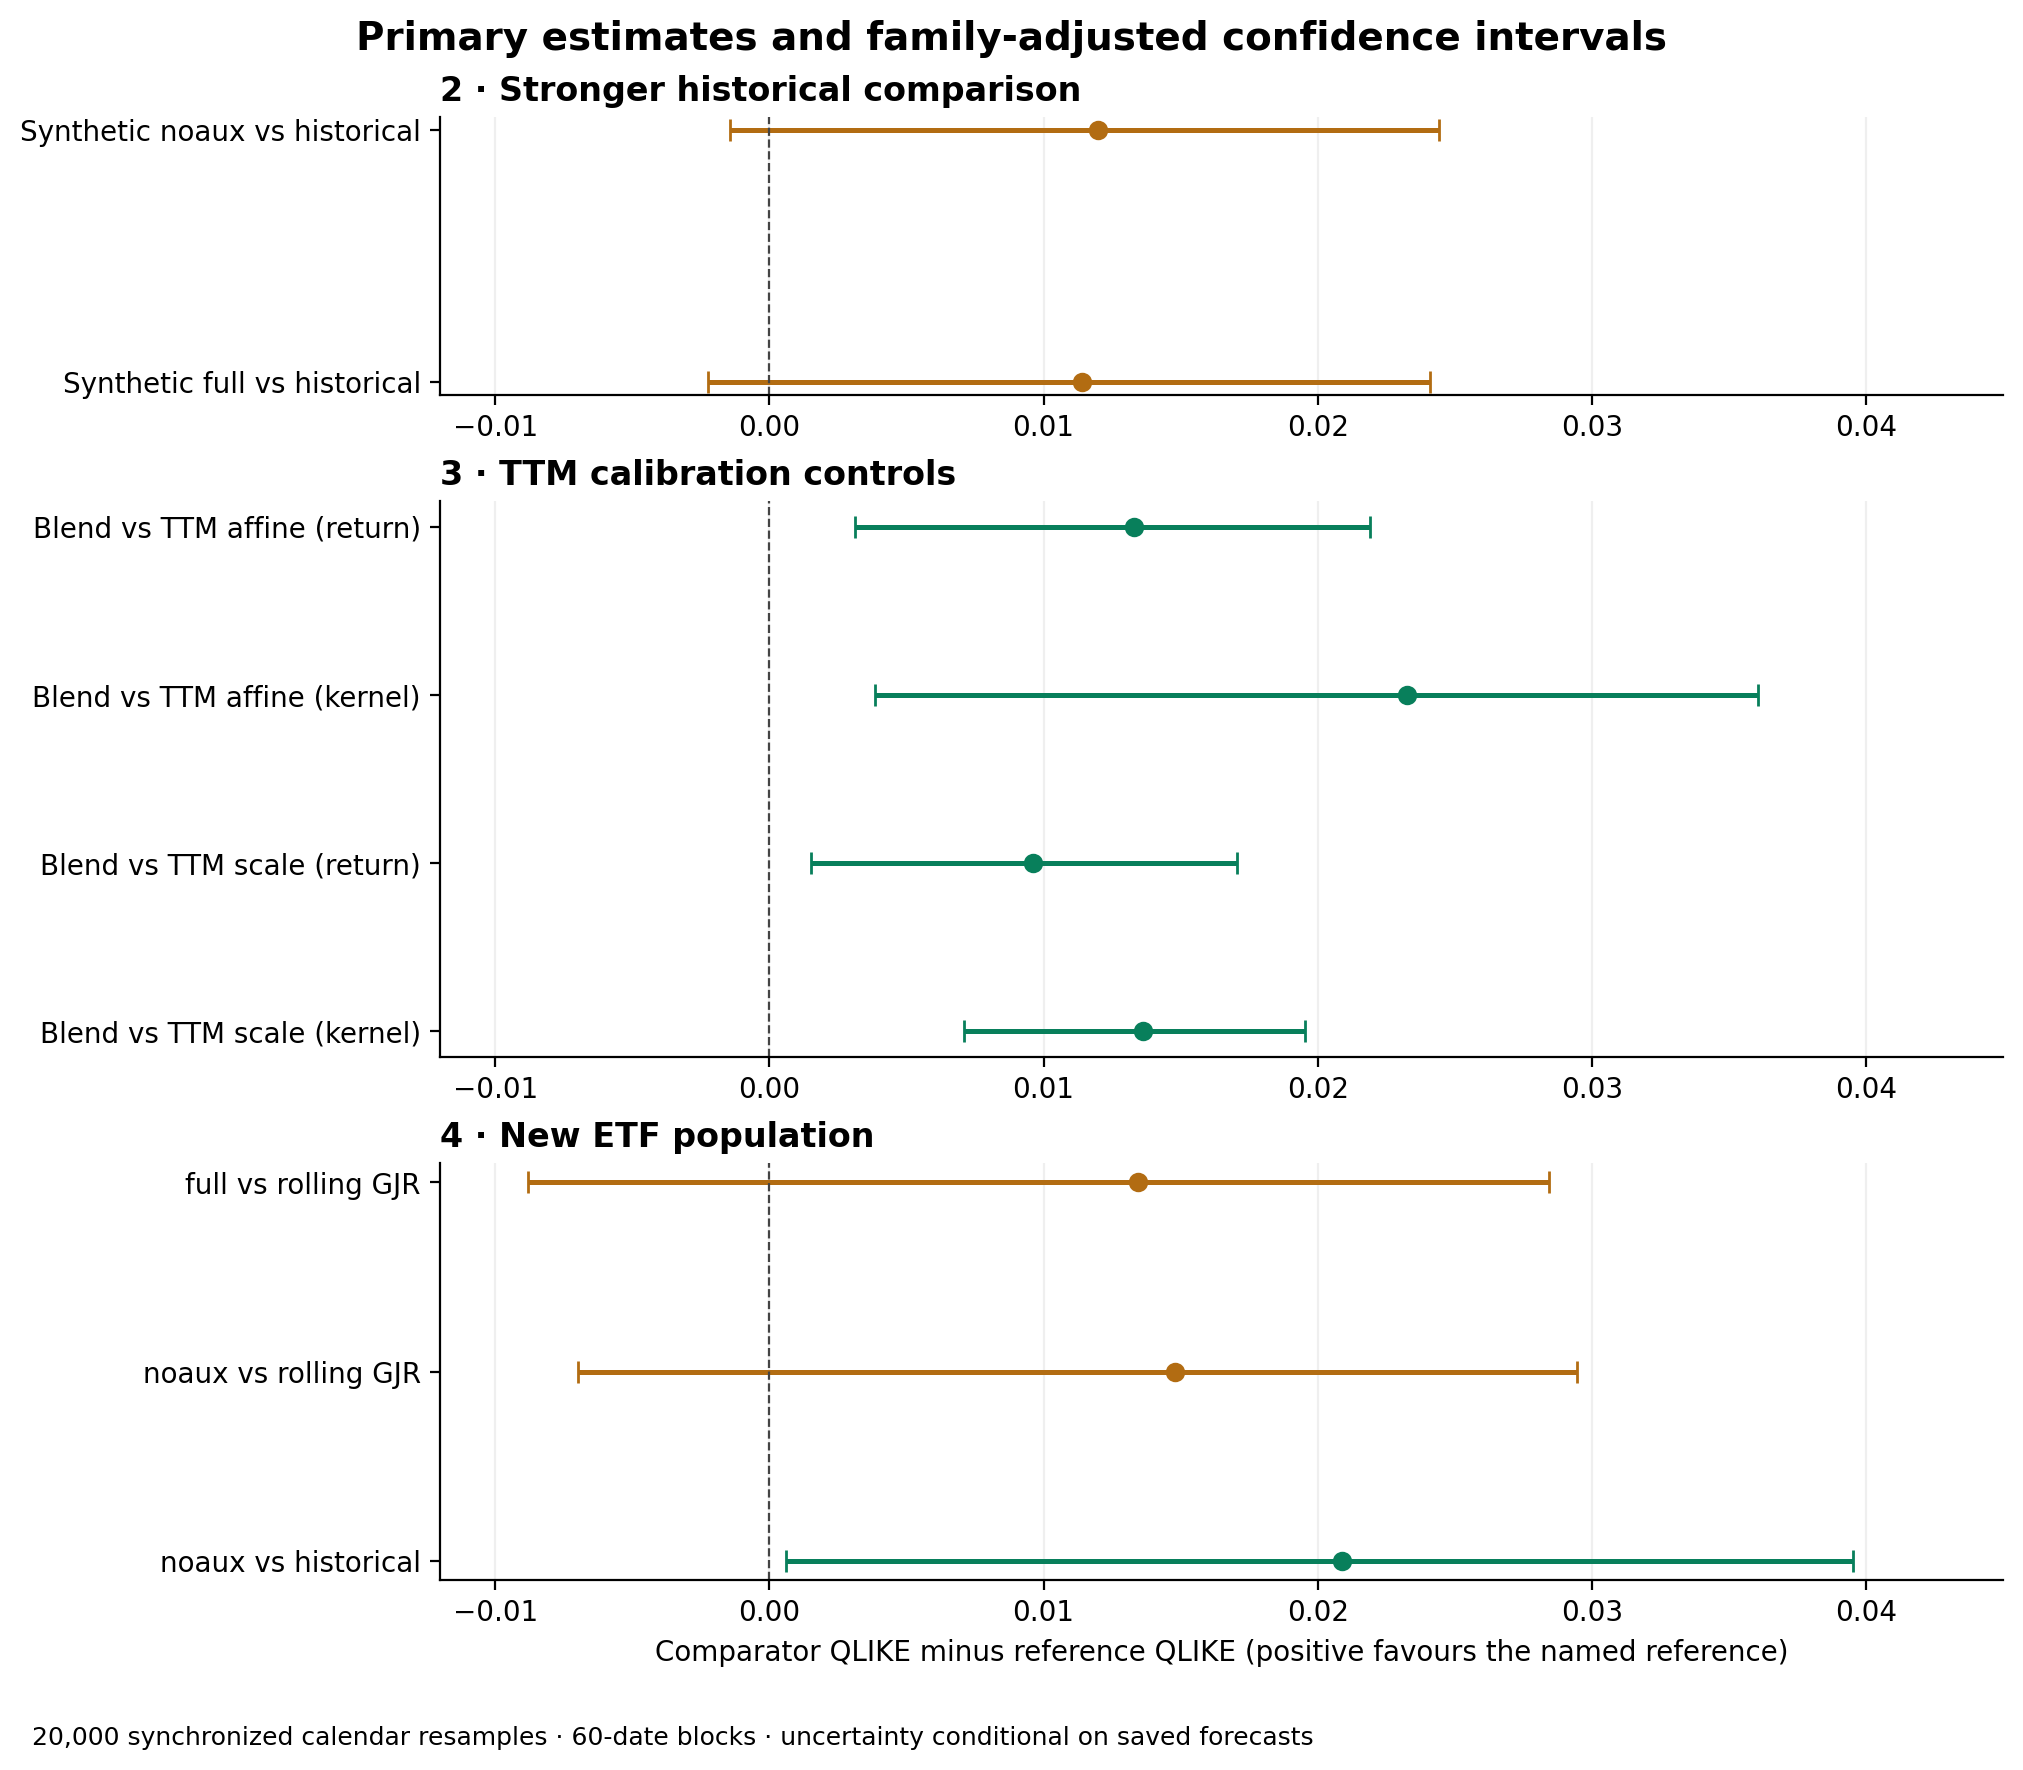
\includegraphics[width=\textwidth]{followup_primary_comparisons.png}
\caption[Primary follow-up gains and family intervals]{Saved follow-up summary: comparator-minus-reference QLIKE gains with Bonferroni family 95\% intervals, 20,000 synchronised resamples and sixty-date blocks. Green intervals are positive; amber intervals include zero. Panel labels 2--4 refer to the follow-up experiment identifiers, not dissertation chapters. Historical contrasts use 50,073 index rows per seed; calibration uses 22,026 keys at each proxy; ETFs use 22,600 rows per model/seed. Families contain two, four and three contrasts respectively. Intervals condition on saved forecasts and exclude retraining, refit re-estimation and research selection.}
\label{fig:followup-primary}
\end{figure}
\FloatBarrier

\subsection{Stronger historical comparison}

We report historical loss minus synthetic loss, so positive values favour the named synthetic procedure. The comparison retains five paired seeds, 28 markets and the original 50,073-row index mask. Neither primary family interval is wholly positive. Native and common-law NLL remain descriptive.

\begin{table}[!htbp]\centering\footnotesize
\setlength{\tabcolsep}{3pt}
\caption[Stronger historical comparison intervals]{Primary historical follow-up comparisons. Sixty-date blocks; ordinary and Bonferroni family intervals are distinct. Holm corrections apply within this family only.}
\label{tab:followup-inference-0}
\begin{tabular}{lrrrrr}
\toprule Contrast & Gain & Ordinary 95\% CI & Family 95\% CI & Holm $p$ & Markets \\
\midrule
Noaux--historical & 0.011966 & $[0.000214,0.022999]$ & $[-0.001440,0.024424]$ & 0.079196 & 20/28 \\
Full--historical & 0.011385 & $[-0.000520,0.022544]$ & $[-0.002243,0.024104]$ & 0.079196 & 19/28 \\
\bottomrule\end{tabular}\end{table}

The new historical seed QLIKE scores are 0.600664, 0.600698, 0.612527, 0.600172 and 0.596363 for seeds 8101--8105. Each retains one QLIKE-above-100 event. Both synthetic gains are positive in all paired seeds, with noaux positive in 20/28 markets and full in 19/28. The ordinary noaux interval excludes zero, but the family interval does not; marginal support therefore does not establish family-level superiority. The original mean 221.292094 and its 15,163 exceptional seed-level forecasts remain failure diagnostics, not the primary source comparison.

\FloatBarrier

\subsection{Causal TTM calibration comparisons}

The reported gain subtracts full VolPFN+TTM loss from control loss, favouring the blend when positive. Both proxies retain the same 22,026 keys and 28 markets, and all four declared contrasts pass their family rule. Raw TTM and GJR+TTM keep their earlier, separate inference.

\begin{table}[!htbp]\centering\footnotesize
\setlength{\tabcolsep}{3pt}
\caption[Causal TTM calibration comparisons intervals]{Primary causal TTM calibration comparisons. Sixty-date blocks; ordinary and Bonferroni family intervals are distinct. Holm corrections apply within this family only.}
\label{tab:followup-inference-1}
\begin{tabular}{lrrrrr}
\toprule Contrast & Gain & Ordinary 95\% CI & Family 95\% CI & Holm $p$ & Markets \\
\midrule
Affine TTM/return & 0.013311 & $[0.005432,0.020228]$ & $[0.003110,0.021917]$ & 0.001800 & 21/28 \\
Affine TTM/RK & 0.023257 & $[0.008463,0.033998]$ & $[0.003842,0.036062]$ & 0.003900 & 28/28 \\
Scale TTM/return & 0.009615 & $[0.003317,0.015530]$ & $[0.001502,0.017042]$ & 0.003900 & 20/28 \\
Scale TTM/RK & 0.013622 & $[0.008571,0.018389]$ & $[0.007095,0.019515]$ & 0.000200 & 25/28 \\
\bottomrule\end{tabular}\end{table}

Every blend seed improves over both controls at both proxies. After primary inspection, a descriptive check removes the first sixty union dates, retaining 20,414 rows. Return/RK QLIKE is 0.701348/0.627509 for the blend, 0.707067/0.641022 for raw TTM, 0.716325/0.652617 for affine TTM and 0.712339/0.642220 for scale TTM. It retains the ordering without new tests or a replacement primary population. Raw controls and the blend have different warm-up forecasts, as specified in Appendix~\ref{sec:followup-methods}.

\FloatBarrier

\subsection{Frozen external ETF comparisons}

Comparator-minus-reference loss favours the reference when positive. The fixed twenty-ETF population supplies 22,600 rows per model and seed. Only noaux--historical passes the complete primary rule; rolling-GJR family intervals both cross zero. Unverified human exposure and overlapping index-study shocks qualify this external population result.

\begin{table}[!htbp]\centering\footnotesize
\setlength{\tabcolsep}{3pt}
\caption[Frozen external ETF comparisons intervals]{Primary frozen external ETF comparisons. Sixty-date blocks; ordinary and Bonferroni family intervals are distinct. Holm corrections apply within this family only.}
\label{tab:followup-inference-2}
\begin{tabular}{lrrrrr}
\toprule Contrast & Gain & Ordinary 95\% CI & Family 95\% CI & Holm $p$ & Markets \\
\midrule
Full--Rolling GJR & 0.013460 & $[-0.004078,0.026624]$ & $[-0.008815,0.028430]$ & 0.100195 & 16/20 \\
Noaux--Rolling GJR & 0.014800 & $[-0.002427,0.027629]$ & $[-0.006986,0.029456]$ & 0.100195 & 16/20 \\
Noaux--Historical & 0.020872 & $[0.004305,0.036359]$ & $[0.000599,0.039524]$ & 0.029999 & 18/20 \\
\bottomrule\end{tabular}\end{table}

All five paired noaux--historical gains are positive: 0.018444, 0.019941, 0.031796, 0.019850 and 0.014327. Both synthetic--GJR contrasts also have positive seed means, but their primary uncertainty remains inconclusive. Eighteen of twenty ETFs favour noaux over historical and sixteen favour each synthetic model over GJR. These descriptive breadth counts are not independent market tests or an added decision gate.

\FloatBarrier

\subsection{Descriptive density endpoints}

Table~\ref{tab:followup-density} reports descriptive native and common-law NLL, with lower values preferred. Fixed synthetic and selected historical weights forecast the index panel; the ETF panel freezes these weights and retains rolling GJR's fitted mean in native scoring. Common scoring uses issued second moment under a zero-mean $t_8$ law. We construct no additional NLL hypothesis family.

\begin{table}[!htbp]\centering\small
\caption[Descriptive follow-up density losses]{Equal-market/seed mean NLL on the exact primary return masks. Historical refers to the new development-selected procedure; the original failure is separately retained in Table~\ref{tab:followup-historical}. Density endpoints are descriptive.}
\label{tab:followup-density}
\begin{tabular}{llrr}
\toprule Population & Procedure & Native NLL & Common $t_8$ NLL \\
\midrule
Indices & Full & 1.178272 & 1.184313 \\
Indices & Historical & 1.202152 & 1.187763 \\
Indices & Noaux & 1.177252 & 1.183908 \\
ETFs & Full & 1.111583 & 1.112836 \\
ETFs & Rolling GJR & 1.117771 & 1.116972 \\
ETFs & Historical & 1.138492 & 1.120480 \\
ETFs & Noaux & 1.111585 & 1.112374 \\
\bottomrule\end{tabular}\end{table}
\FloatBarrier

\subsection{Calendar-block sensitivities and complete decisions}

Table~\ref{tab:followup-sensitivity} repeats correction separately for each family's twenty- and 120-date alternatives. These are sensitivities rather than new primary tests. Historical superiority stays unresolved, all calibration contrasts remain supported, and ETF noaux--historical retains support. At twenty-date blocks the ETF--GJR adjusted probabilities both fall below 0.05, but their family intervals still cross zero. Selecting that block alone would therefore misstate the complete decision rule.

\begingroup
\small
\setlength{\tabcolsep}{4pt}
\begin{longtable}{@{}>{\raggedright\arraybackslash}p{4.5cm}rrrr@{}}
\caption[Follow-up block sensitivities]{Family-adjusted probabilities and intervals under the two alternative calendar block lengths. Gains equal the corresponding primary estimates. The two historical, four calibration and three ETF families remain separate.}\label{tab:followup-sensitivity}\\
\toprule Contrast & Block & Holm $p$ & Family 95\% interval & Support \\
\midrule\endfirsthead
\toprule Contrast & Block & Holm $p$ & Family 95\% interval & Support \\
\midrule\endhead
Index Noaux--historical & 20 & 0.079296 & $[-0.001471,0.024352]$ & No \\
Index Full--historical & 20 & 0.079296 & $[-0.002243,0.023973]$ & No \\
Index Noaux--historical & 120 & 0.052597 & $[-0.000512,0.023722]$ & No \\
Index Full--historical & 120 & 0.052597 & $[-0.001445,0.023395]$ & No \\
Affine TTM/return & 20 & 0.004650 & $[0.000800,0.023263]$ & Yes \\
Affine TTM/RK & 20 & 0.001800 & $[0.007342,0.033734]$ & Yes \\
Scale TTM/return & 20 & 0.004400 & $[0.001637,0.017376]$ & Yes \\
Scale TTM/RK & 20 & 0.000200 & $[0.008268,0.018666]$ & Yes \\
Affine TTM/return & 120 & 0.001050 & $[0.003365,0.021706]$ & Yes \\
Affine TTM/RK & 120 & 0.004300 & $[0.002809,0.037259]$ & Yes \\
Scale TTM/return & 120 & 0.004300 & $[0.001430,0.016837]$ & Yes \\
Scale TTM/RK & 120 & 0.000200 & $[0.006015,0.020360]$ & Yes \\
ETF Full--Rolling GJR & 20 & 0.030298 & $[-0.003162,0.025859]$ & No \\
ETF Noaux--Rolling GJR & 20 & 0.030298 & $[-0.001677,0.027039]$ & No \\
ETF Noaux--Historical & 20 & 0.010349 & $[0.003599,0.037269]$ & Yes \\
ETF Full--Rolling GJR & 120 & 0.129194 & $[-0.009300,0.029612]$ & No \\
ETF Noaux--Rolling GJR & 120 & 0.129194 & $[-0.007566,0.030507]$ & No \\
ETF Noaux--Historical & 120 & 0.037648 & $[0.000840,0.040642]$ & Yes \\
\bottomrule\end{longtable}
\endgroup

\subsection{Result identities and preservation}

The authoritative summaries are \path{historical_analysis_v1/}, \path{ttm_control_v1/} and \path{external_confirmation_v1/}. Each retains \path{leaderboard.csv}, \path{statistics.json}, \path{protocol.json}, \path{VERIFICATION.json} and \path{FINAL_RECEIPT.json}. The ETF directory also records execution classification, input checkpoints, original-weight checks, CPU replay and GJR causality. Source/receipt checks preserve the original inputs and distinguish serialization repair from scientific changes. Root \path{ORIGINALS_PRESERVED.json} binds consumed prior inputs; this manuscript revision separately records hashes of prior dissertation files and consumed completed results.

The original follow-up revision incorporated completed records without repeating training, forecasting, fitting or resampling. It narrowed the interpretation of historical failure and addressed the stated calibration-control gap, retaining negative and unresolved comparisons. The four prose-revision stages preserve those studies and qualifications. Implementation verification cannot establish untouched human exposure or independence from research selection.

